\documentclass[aspectratio=169,10pt]{beamer}
\usetheme{metropolis}
\usepackage{amsmath,amssymb,bm}
\usepackage{siunitx}
\usepackage{booktabs}
\usepackage{tikz}
\usetikzlibrary{arrows.meta,calc,positioning}
\sisetup{per-mode=symbol,detect-all}
\metroset{numbering=fraction,progressbar=frametitle,block=fill}
\tikzset{capt/.style={text width=5.2cm,align=center}}
\hypersetup{colorlinks=true,urlcolor=blue!60!black,linkcolor=.}
% ITU logo on every frame (top-right): white version on the dark title bar, navy on the title page.
\usepackage{tikz}
\addtobeamertemplate{frametitle}{}{%
  \begin{tikzpicture}[remember picture,overlay]
    \node[anchor=north east,yshift=-1.5pt,xshift=-6pt] at (current page.north east) {
\includegraphics[height=0.7cm]{logos/itu_logo_beyaz.pdf}};
  \end{tikzpicture}}
\titlegraphic{\hfill
\includegraphics[height=1.6cm]{logos/itu_logo_laci.pdf}}

\title{Lecture 1: Mechanical Design in the Aerospace Context}
\subtitle{UCK 364E Design of Machine Elements}
\author{Prof.\ Dr.\ Onur Tunçer}
\institute{Department of Aeronautical Engineering, Istanbul Technical University}
\date{Fall 2026}

\begin{document}
\maketitle

\begin{frame}{Today}
\begin{enumerate}
  \item What is a machine element? Why is this course different for you?
  \item Loads, factors and margins the way the certification codes define them
  \item Design allowables: A-, B-, S-basis
  \item Stress--strain review: 3-D stress, yield criteria, stress concentration
  \item The design process and the three questions every element must answer
  \item Selecting aerospace materials: aluminium, titanium, steels, corrosion, temperature
  \item The drawing as a contract: tolerances, fits, finish, standard parts
  \item Introduction to standards, with bolt and nut standards as the worked example
  \item Design principles and the errors that cause accidents
  \item Three worked examples
\end{enumerate}
\end{frame}

\section{Machine elements on an aircraft}

\begin{frame}{What is a machine element?}
\begin{itemize}
  \item A \alert{standardised load-carrying component} with established design rules, standards and catalogue data
  \item Fasteners, rivets, welds, bonds, keys, splines, springs, bearings, shafts, gears
  \item You will rarely invent one; you will \alert{select, size and integrate} them
  \item Service failures are almost always failures of an element or a joint, not of a bulk panel
\end{itemize}
\end{frame}

\begin{frame}{Where they live on an airframe}
\small
\begin{tabular}{@{}lll@{}}
\toprule
Element & Aircraft location & Governing concern \\
\midrule
Bolts, Hi-Loks, rivets & Fittings, lap joints, frames & Fatigue, preload, bearing/bypass \\
Lugs and fittings & Wing root, gear trunnion, engine mount & Fitting factor, fatigue, fretting \\
Welds & Steel-tube fuselage, engine mount & Weld fatigue class, NDT \\
Adhesive bonds & Sandwich, doublers, repairs, spacecraft & Peel, environment, outgassing \\
Splines, keys, fits & Accessory drives, actuators & Fretting, tolerance stack-up \\
Springs & Landing gear, valves, latches & Fatigue, surge, relaxation \\
Rolling bearings & Wheels, hinges, actuators, gearboxes & $L_{10}$ life, spectrum \\
Gears & Accessory gearbox, rotor transmission & Tooth bending/contact fatigue \\
\bottomrule
\end{tabular}
\vspace{4pt}
\begin{block}{Consequence for this course}
Fatigue first, joints in the middle, bearings and gears last.
\end{block}
\end{frame}



\section{Loads, factors and margins}


\begin{frame}{First, the alphabet: who writes the rules?}
\footnotesize
\begin{columns}[T]
\column{0.5\textwidth}
\textbf{Europe --- EASA}
\begin{itemize}
  \item \alert{CS} = \emph{Certification Specifications}: the airworthiness code an aircraft type must meet
  \item CS-25 large aeroplanes, CS-23 small aeroplanes, CS-27/29 rotorcraft, CS-E engines, CS-P propellers
  \item \textbf{Book 1}: binding requirements (e.g.\ CS 25.303); \textbf{Book 2}: \alert{AMC}, Acceptable Means of Compliance (how to show you meet them)
\end{itemize}
\column{0.5\textwidth}
\textbf{USA --- FAA}
\begin{itemize}
  \item \alert{FAR} = Federal Aviation Regulations (14 CFR); Parts 25, 23, 27/29, 33 mirror the CS numbering paragraph for paragraph
  \item \alert{AC} = Advisory Circular: FAA guidance, the counterpart of AMC (e.g.\ AC 25.571-1D on fatigue and damage tolerance)
\end{itemize}
\end{columns}
\vspace{4pt}
\begin{block}{How to read a reference like ``CS-25.625''}
CS-25 is the document, \S625 is the paragraph: ``fitting factors''. The same rule is FAR 25.625. In Türkiye, SHGM adopts the EASA CS texts, so CS is what you will design to.
\end{block}
\scriptsize Free and official --- bookmark: CS-25 (Easy Access Rules, CS + AMC): \href{https://www.easa.europa.eu/en/document-library/easy-access-rules/online-publications/easy-access-rules-large-aeroplanes-cs-25}{easa.europa.eu \textrightarrow\ Easy Access Rules for Large Aeroplanes (CS-25)}\\
FAR Part 25 (eCFR, 14 CFR 25): \href{https://www.ecfr.gov/current/title-14/chapter-I/subchapter-C/part-25}{ecfr.gov \textrightarrow\ Title 14, Part 25}
\end{frame}

\begin{frame}{The design inequality}
\begin{equation*}
  \underbrace{\text{applied}}_{\text{loads analysis}}\times\underbrace{\text{factors}}_{\text{code}}\;\le\;\underbrace{\text{allowable}}_{\text{MMPDS}}
\end{equation*}
\begin{itemize}
  \item \alert{Limit load} (CS-25.301): max.\ expected in service; no detrimental permanent deformation (25.305)
  \item \alert{Ultimate load} = limit $\times$ FS, FS $=1.5$ (25.303); carry for \SI{3}{s} without failure
  \item In aerospace the factor of safety is \alert{prescribed}, not chosen
\end{itemize}
\end{frame}

\begin{frame}{Special factors (CS-25.619--625)}
Applied \emph{in addition} to 1.5 whenever strength is uncertain or may deteriorate:
\begin{itemize}
  \item \alert{Fitting factor 1.15} (25.625) on any part transferring load between members, its attachments and bearing surfaces\\
        --- not on continuous plating joints, welded joints
  \item Casting factor 1.25--2.0 (25.621), depending on inspection
  \item Bearing factor (25.623) for free-fit parts under pounding/vibration
  \item Fatigue is \emph{not} a factor: handled by 25.571
\end{itemize}
\end{frame}

\begin{frame}{Margin of safety}
\begin{equation*}
  \mathrm{MS}=\frac{\text{allowable}}{\text{applied}\times\mathrm{FS}\times(\text{special factors})}-1\;\ge 0
\end{equation*}
\begin{itemize}
  \item Ultimate margin: $F_{tu},F_{su},F_{bru}$ with FS $=1.5$
  \item Yield margin: $F_{ty},F_{bry}$ with FS $=1.0$ at limit load
  \item Smaller governs; MS $\approx 0$ is efficient, MS $\gg 0$ is weight, MS $<0$ is a finding
\end{itemize}
\begin{block}{Shigley vs.\ CS-25}
Shigley: $n = S/\sigma$ chosen by designer (1.5--4, Pugsley). Airframe: FS fixed, loads certified, allowables statistical, margin reported.
\end{block}
\end{frame}

\begin{frame}{Design allowables: A-, B-, S-basis (CS-25.613, MMPDS)}
\begin{itemize}
  \item \alert{A-basis}: 99\% exceed, 95\% confidence --- single load path
  \item \alert{B-basis}: 90\% exceed, 95\% confidence --- redundant structure
  \item \alert{S-basis}: specification minimum, no statistics
\end{itemize}
\vspace{4pt}
\small
\begin{tabular}{@{}llS[table-format=4]S[table-format=4]S[table-format=3]l@{}}
\toprule
Alloy & Form & {$F_{tu}$} & {$F_{ty}$} & {$F_{su}$} & Use \\
\midrule
2024-T3 & Sheet & 434 & 289 & 262 & Fuselage skin \\
7075-T6 & Sheet & 524 & 462 & 317 & Wing skin, spars \\
Ti-6Al-4V & Bar & 896 & 827 & 545 & Gear, mounts, fasteners \\
4340 (1800 HT) & Bar & 1793 & 1517 & 1076 & Landing gear \\
15-5PH H1025 & Bar & 1069 & 1000 & 655 & Fittings, actuators \\
\bottomrule
\end{tabular}
\hfill\tiny (MPa, approx.\ B-basis, classroom only)
\end{frame}

\section{Stress--strain review}

\begin{frame}{Principal stresses and Mohr's circle (plane stress)}
\begin{columns}
\column{0.55\textwidth}
\begin{align*}
\sigma_{1,2} &= \frac{\sigma_x+\sigma_y}{2}\pm\sqrt{\Big(\frac{\sigma_x-\sigma_y}{2}\Big)^2+\tau_{xy}^2}\\
\tau_{\max} &= \sqrt{\Big(\frac{\sigma_x-\sigma_y}{2}\Big)^2+\tau_{xy}^2}
\end{align*}
Third principal stress is zero: the true $\tau_{\max}$ may be $\sigma_1/2$.
\column{0.45\textwidth}
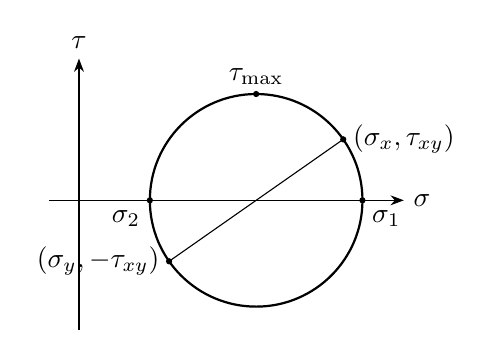
\begin{tikzpicture}[scale=0.75,>=Stealth]
  \draw[->] (-0.5,0) -- (5.5,0) node[right] {$\sigma$};
  \draw[->] (0,-2.2) -- (0,2.4) node[above] {$\tau$};
  \coordinate (C) at (3,0);
  \draw[thick] (C) circle (1.8);
  \fill (4.8,0) circle (1.5pt) node[below right] {$\sigma_1$};
  \fill (1.2,0) circle (1.5pt) node[below left] {$\sigma_2$};
  \fill (3,1.8) circle (1.5pt) node[above] {$\tau_{\max}$};
  \coordinate (X) at ($(C)+(35:1.8)$);
  \coordinate (Y) at ($(C)+(215:1.8)$);
  \fill (X) circle (1.5pt) node[right] {$(\sigma_x,\tau_{xy})$};
  \fill (Y) circle (1.5pt) node[left] {$(\sigma_y,-\tau_{xy})$};
  \draw (X) -- (Y);
\end{tikzpicture}
\end{columns}
\end{frame}

\begin{frame}{Static failure criteria for ductile metals}
\begin{align*}
\text{Tresca:}\quad & \sigma_1-\sigma_3\le S_y/n\\
\text{von Mises:}\quad & \sigma'=\sqrt{\tfrac12\big[(\sigma_1-\sigma_2)^2+(\sigma_2-\sigma_3)^2+(\sigma_3-\sigma_1)^2\big]}\le S_y/n\\
& \sigma'=\sqrt{\sigma_x^2+3\tau_{xy}^2}\quad(\text{axial}+\text{torsion})
\end{align*}
\begin{itemize}
  \item Von Mises is the airframe standard; Tresca up to 15\% conservative
  \item Brittle materials (castings, some composites): Coulomb--Mohr --- not used here
\end{itemize}
\end{frame}

\begin{frame}{Stress concentration}
\begin{itemize}
  \item $\sigma_{\max}=K_t\,\sigma_{\text{nom}}$, $K_t$ from Peterson (Pilkey)
  \item Circular hole, infinite plate, uniaxial: $K_t=3$; finite width $d/w=0.2$: $K_t\approx2.5$
  \item Static ductile design: usually ignore $K_t$ (local yielding)
  \item Fatigue: decisive, through $K_f$
\end{itemize}
\begin{alertblock}{Every lug, fastener hole and window corner is a stress concentration}
de Havilland Comet, 1954: square-cornered ADF window cut-outs, pressurisation fatigue.
\end{alertblock}
\end{frame}

\begin{frame}{Formulae you will use throughout the course}
\small
\begin{tabular}{@{}lll@{}}
\toprule
Case & Stress & Note \\
\midrule
Axial & $\sigma=P/A$ & net area at holes \\
Bending & $\sigma=My/I$ & $Z=I/c$ \\
Torsion & $\tau=Tr/J$, $J=\pi d^4/32$ & \\
Transverse shear & $\tau=VQ/(Ib)$ & $\tfrac32 V/A$ rect., $\tfrac43 V/A$ circ. \\
Bearing & $\sigma_{br}=P/(dt)$ & projected area \\
Thin cylinder & $\sigma_\theta=pr/t$, $\sigma_z=pr/2t$ & fuselage \\
Thin sphere & $\sigma=pr/2t$ & bulkhead, tank \\
Hertz, sphere/plane & $p_{\max}=3F/(2\pi a^2)$ & bearings \\
\bottomrule
\end{tabular}
\vspace{6pt}

Ramberg--Osgood: $\varepsilon=\sigma/E+0.002(\sigma/F_{ty})^n$, $n\approx10$--15 (2024), 20--25 (7075)
\end{frame}


\section{The design process}

\begin{frame}{From requirement to certified part}
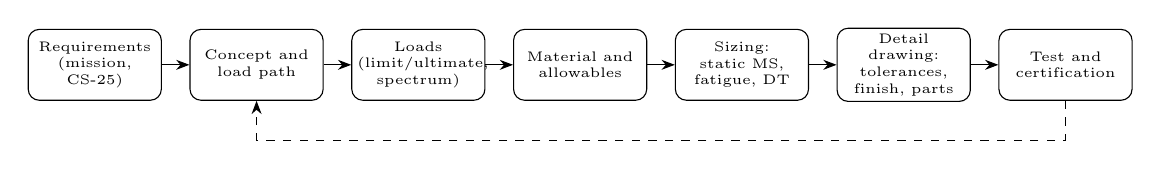
\begin{tikzpicture}[>=Stealth,node distance=0.35cm,every node/.style={draw,rounded corners,align=center,font=\tiny,minimum height=0.9cm,text width=1.55cm,inner sep=2pt}]
\node (a) {Requirements\\ (mission, CS-25)};
\node[right=of a] (b) {Concept and\\ load path};
\node[right=of b] (c) {Loads\\ (limit/ultimate,\\ spectrum)};
\node[right=of c] (d) {Material and\\ allowables};
\node[right=of d] (e) {Sizing:\\ static MS,\\ fatigue, DT};
\node[right=of e] (f) {Detail drawing:\\ tolerances,\\ finish, parts};
\node[right=of f] (g) {Test and\\ certification};
\foreach \x/\y in {a/b,b/c,c/d,d/e,e/f,f/g} \draw[->] (\x) -- (\y);
\draw[->,dashed] (g.south) -- ++(0,-0.5) -| (b.south);
\end{tikzpicture}
\vspace{6pt}
\begin{itemize}
  \item This course lives in boxes 4--6 and reaches into box 7
  \item 80\% of the cost is committed by the time the drawing is released; most errors are born in boxes 2 and 6
\end{itemize}
\end{frame}

\begin{frame}{The three questions every element must answer}
\begin{enumerate}
  \item \alert{Strength}: does it carry ultimate load with positive margin? (static)
  \item \alert{Life}: does it survive the load spectrum for the design service goal with the required inspection scheme? (fatigue and damage tolerance)
  \item \alert{Function}: does it keep doing its job --- no loosening, no fretting, no jamming, no leak, no excessive wear --- over the life?
\end{enumerate}
\begin{block}{}
Most failures in service are in categories 2 and 3. Category 1 is the one your textbook spends the most pages on.
\end{block}
\end{frame}

\section{Selecting aerospace materials}

\begin{frame}{What drives material choice for an aircraft element?}
\begin{columns}[T]
\column{0.5\textwidth}
\textbf{Performance}
\begin{itemize}
  \item Specific strength $F_{tu}/\rho$, specific stiffness $E/\rho$
  \item Fatigue strength and crack-growth rate $\mathrm d a/\mathrm d N$
  \item Fracture toughness $K_{Ic}$ (residual strength)
  \item Temperature: strength retention, creep
  \item Corrosion: general, stress-corrosion, galvanic
\end{itemize}
\column{0.5\textwidth}
\textbf{Practicality}
\begin{itemize}
  \item Availability in the required form (sheet, plate, forging, bar)
  \item Machinability, formability, weldability
  \item Certified data: is it in MMPDS?
  \item Cost, lead time, supplier qualification
  \item Inspectability (NDT) and repairability
\end{itemize}
\end{columns}
\vspace{4pt}
\small For a \emph{machine element} the questions narrow further: bearing strength, thread strength, wear, and compatibility with the mating part.
\end{frame}

\begin{frame}{Specific properties: the first cut}
\centering
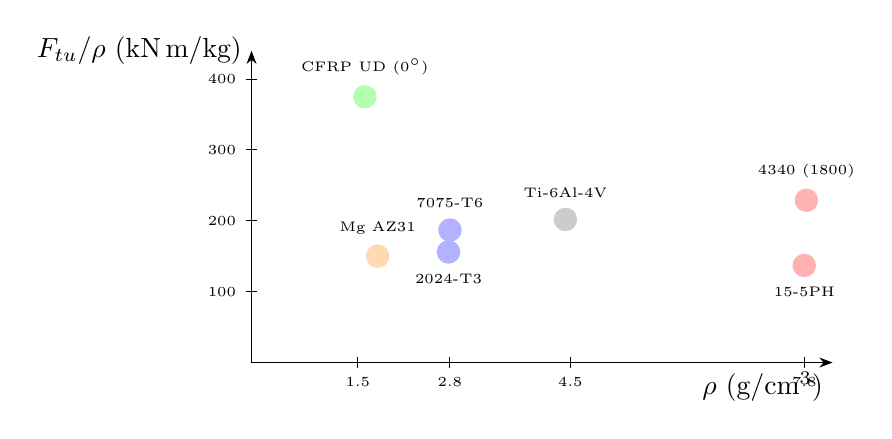
\begin{tikzpicture}[scale=0.9,>=Stealth]
\draw[->] (0,0) -- (8.2,0) node[below left] {$\rho$ (g/cm$^3$)};
\draw[->] (0,0) -- (0,4.4) node[left] {$F_{tu}/\rho$ (kN\,m/kg)};
\foreach \x/\l in {1.5/1.5,2.8/2.8,4.5/4.5,7.8/7.8} \draw (\x,0.08)--(\x,-0.08) node[below,font=\tiny] {\l};
\foreach \y/\l in {1/100,2/200,3/300,4/400} \draw (0.08,\y)--(-0.08,\y) node[left,font=\tiny] {\l};
\node[fill=blue!30,circle,inner sep=3pt,label={[font=\tiny]above:7075-T6}] at (2.8,1.87) {};
\node[fill=blue!30,circle,inner sep=3pt,label={[font=\tiny]below:2024-T3}] at (2.78,1.56) {};
\node[fill=gray!40,circle,inner sep=3pt,label={[font=\tiny]above:Ti-6Al-4V}] at (4.43,2.02) {};
\node[fill=red!30,circle,inner sep=3pt,label={[font=\tiny]above:4340 (1800)}] at (7.83,2.29) {};
\node[fill=red!30,circle,inner sep=3pt,label={[font=\tiny]below:15-5PH}] at (7.8,1.37) {};
\node[fill=green!30,circle,inner sep=3pt,label={[font=\tiny]above:CFRP UD (0$^\circ$)}] at (1.6,3.75) {};
\node[fill=orange!30,circle,inner sep=3pt,label={[font=\tiny]above:Mg AZ31}] at (1.78,1.5) {};
\end{tikzpicture}
\vspace{-4pt}

\small Specific strength alone says ``use composites and titanium''. Fatigue, toughness, bearing strength, cost and joinability say otherwise for most machine elements.
\end{frame}

\begin{frame}{Aluminium alloys: the two families}
\begin{columns}[T]
\column{0.5\textwidth}
\textbf{2xxx (Al--Cu): damage tolerant}
\begin{itemize}
  \item 2024-T3, 2524-T3: fuselage skin, lower wing skin
  \item Lower strength, higher toughness, slower crack growth
  \item Poor corrosion resistance --- clad or anodised
  \item Not fusion-weldable in practice
\end{itemize}
\textbf{7xxx (Al--Zn--Mg--Cu): high strength}
\begin{itemize}
  \item 7075-T6, 7050-T7451, 7150: upper wing skin, spars, ribs, fittings
  \item T6 is SCC-prone in the short-transverse direction $\Rightarrow$ T73/T74 overaged tempers for thick fittings
\end{itemize}
\column{0.5\textwidth}
\textbf{Rules of thumb}
\begin{itemize}
  \item Tension-fatigue dominated $\rightarrow$ 2xxx
  \item Compression/strength dominated $\rightarrow$ 7xxx
  \item Thick section, complex fitting $\rightarrow$ 7050/7085 plate or forging, T74
  \item Weldable structural Al: 6061-T6, 5083 (much weaker), 2219 (launch vehicles), Al--Li 2195/2099
\end{itemize}
\begin{alertblock}{Direction matters}
L, LT, ST properties differ; ST toughness of thick 7075-T6 plate can be half of L. Grain direction is a drawing note.
\end{alertblock}
\end{columns}
\end{frame}

\begin{frame}{Titanium, steels, and the rest}
\scriptsize
\begin{tabular}{@{}p{2.4cm}p{5.6cm}p{6.2cm}@{}}
\toprule
Material & Where & Why / watch out \\
\midrule
Ti-6Al-4V & Landing-gear parts, engine mounts, pylon fittings, fasteners, anything touching CFRP & Galvanically compatible with carbon; \SI{400}{\celsius} capable; expensive; notch-sensitive; galling in threads (needs lubricant) \\
Ti-10V-2Fe-3Al, Ti-5553 & Landing-gear forgings & Higher strength, replaces steel with weight saving \\
4340, 300M & Landing-gear main structure, high-load bolts & \SIrange{1800}{2000}{MPa}; hydrogen embrittlement from plating; must be shot-peened, cadmium/Zn--Ni plated \\
15-5PH, 17-4PH, PH13-8Mo & Fittings, actuator housings, pins & Corrosion-resistant, good toughness, easier to machine than 4340 \\
A286, Inconel 718 & Hot-section fasteners, exhaust, engine & Strength to \SIrange{650}{700}{\celsius} \\
Bronze, Al--Ni--bronze & Bushings, sliding surfaces & Bearing pairs with steel pins \\
CFRP / GFRP & Skins, spars, control surfaces & Element course cares about the \emph{joint} to it: bearing/bypass, galvanic isolation \\
\bottomrule
\end{tabular}
\end{frame}

\begin{frame}{Corrosion and compatibility --- the silent element killer}
\begin{columns}[T]
\column{0.55\textwidth}
\begin{itemize}
  \item \alert{Galvanic}: Al in contact with CFRP or steel corrodes --- use Ti fasteners, glass-fibre isolation ply, sealant, cadmium or Zn--Ni plated steel
  \item \alert{Stress-corrosion cracking}: 7075-T6 ST direction, high-strength steels; sustained tensile stress + environment
  \item \alert{Crevice / trap corrosion}: any pocket that holds moisture --- drain holes, faying-surface sealant
  \item \alert{Fretting}: micro-slip at clamped interfaces cuts fatigue life by 3--10$\times$
  \item \alert{Hydrogen embrittlement}: plated high-strength steel must be baked
\end{itemize}
\column{0.45\textwidth}
\begin{block}{Design checklist on every drawing}
\begin{itemize}
  \item Finish and plating spec called out
  \item Dissimilar-metal isolation specified
  \item Sealant at faying surfaces
  \item Drainage path
  \item Grain direction on 7xxx forgings
\end{itemize}
\end{block}
\end{columns}
\end{frame}

\begin{frame}{Temperature: where each material stops}
\centering
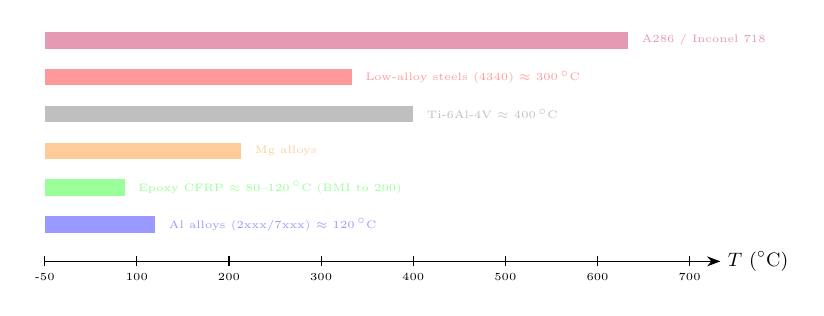
\begin{tikzpicture}[>=Stealth,scale=0.78,every node/.style={transform shape}]
\draw[->] (0,0) -- (11,0) node[right,font=\small] {$T$ (\si{\celsius})};
\foreach \x/\l in {0/-50,1.5/100,3/200,4.5/300,6/400,7.5/500,9/600,10.5/700} \draw (\x,0.08)--(\x,-0.08) node[below,font=\tiny] {\l};
\draw[line width=6pt,blue!40] (0,0.6) -- (1.8,0.6) node[right,font=\tiny] {Al alloys (2xxx/7xxx) $\approx$ \SI{120}{\celsius}};
\draw[line width=6pt,green!40] (0,1.2) -- (1.3,1.2) node[right,font=\tiny] {Epoxy CFRP $\approx$ \SI{80}{}--\SI{120}{\celsius} (BMI to 200)};
\draw[line width=6pt,orange!40] (0,1.8) -- (3.2,1.8) node[right,font=\tiny] {Mg alloys};
\draw[line width=6pt,gray!50] (0,2.4) -- (6,2.4) node[right,font=\tiny] {Ti-6Al-4V $\approx$ \SI{400}{\celsius}};
\draw[line width=6pt,red!40] (0,3.0) -- (5,3.0) node[right,font=\tiny] {Low-alloy steels (4340) $\approx$ \SI{300}{\celsius}};
\draw[line width=6pt,purple!40] (0,3.6) -- (9.5,3.6) node[right,font=\tiny] {A286 / Inconel 718};
\end{tikzpicture}
\vspace{4pt}

\small Brakes, engine bays, anti-ice ducts, supersonic leading edges, re-entry: the element next to the heat source dictates the material and often the whole joint design.
\end{frame}

\begin{frame}{Material selection, worked quickly: a landing-gear pintle pin}
\begin{itemize}
  \item Load: high, cyclic, with bending; bearing against bushings; must not corrode in wheel-well spray
  \item Candidates: 4340/300M (highest strength, needs plating and peening), 15-5PH (corrosion-resistant, \SI{1070}{MPa}), Ti-6Al-4V (light, but galls and has low bearing strength)
  \item Choice on most aircraft: \alert{300M or 4340, Cd or Zn--Ni plated, shot-peened}, running in Al--Ni--bronze bushings --- strength and bearing win over corrosion, which is handled by process
  \item On a small UAV: 15-5PH or 17-4PH --- no plating line, corrosion resistant, strength sufficient
\end{itemize}
\begin{block}{Pattern}
For \emph{elements} (pins, bolts, gears, springs, bearings) the material is usually a steel; aluminium and titanium dominate the \emph{members} they connect.
\end{block}
\end{frame}

\section{The drawing as a contract}

\begin{frame}{What a machine-element drawing must convey}
A drawing is the legal and technical definition of the part. For an element it must carry, beyond geometry:
\begin{columns}[T]
\column{0.5\textwidth}
\begin{itemize}
  \item Material spec and temper (AMS/EN number, not ``7075'')
  \item Grain direction for forgings and thick plate
  \item Dimensional tolerances and \alert{fits} (ISO 286)
  \item Geometric tolerances (ASME Y14.5 / ISO 1101)
  \item Surface finish ($R_a$) where fatigue or sliding matters
\end{itemize}
\column{0.5\textwidth}
\begin{itemize}
  \item Heat treatment, plating, peening, sealant, primer
  \item Standard parts by part number (NAS6204-10, MS21042-4)
  \item Torque or preload for fasteners
  \item Edge breaks, fillet radii (never ``sharp'')
  \item Inspection requirements (NDT class)
\end{itemize}
\end{columns}
\vspace{4pt}
\small You already read drawings (first year). In this course you will \emph{write} the element-specific notes above.
\end{frame}

\begin{frame}{Tolerances and fits in one slide}
\begin{columns}[T]
\column{0.5\textwidth}
\textbf{ISO 286 designation} \quad $\varnothing 20\,\mathrm{H7/g6}$
\begin{itemize}
  \item Letter = position of tolerance zone (H: hole at nominal; g, h, k, n, p: shaft below/at/above)
  \item Number = grade (IT7 $\approx$ \SI{21}{\micro m} at $\varnothing 20$)
  \item Clearance (H7/g6, H7/f7), transition (H7/k6), interference (H7/p6, H7/s6)
\end{itemize}
\textbf{Why you care}
\begin{itemize}
  \item Bearing seats: wrong fit $\rightarrow$ ring creep or preload loss
  \item Pins in lugs: clearance $\rightarrow$ hammering; interference $\rightarrow$ fatigue benefit
\end{itemize}
\column{0.5\textwidth}
\textbf{GD\&T you will meet}
\begin{itemize}
  \item Position of hole patterns (fastener fit-up)
  \item Perpendicularity of bearing bores
  \item Concentricity/runout of shafts
  \item Flatness of faying surfaces (preload, sealing)
\end{itemize}
\textbf{Surface finish}
\begin{itemize}
  \item $R_a$ \SIrange{0.4}{0.8}{\micro m} on fatigue-critical radii
  \item Machining marks across the load $\rightarrow$ crack starters
\end{itemize}
\end{columns}
\end{frame}


\begin{frame}{Example: detail drawing of a lug fitting (what the notes do)}
\centering
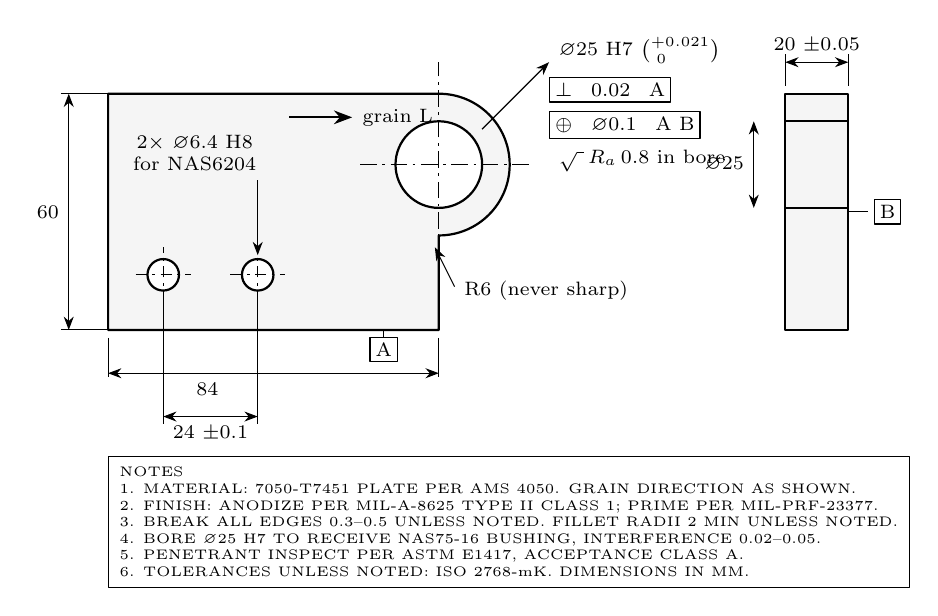
\begin{tikzpicture}[scale=1.0,>=Stealth,line join=round,font=\scriptsize]
% --- front view: lug plate
\draw[thick,fill=gray!8] (0,0) -- (4.2,0) -- (4.2,1.2) arc (-90:90:0.9) -- (0,3.0) -- cycle;
\draw[thick,fill=white] (4.2,2.1) circle (0.55);
\draw[dash pattern=on 6pt off 2pt on 1pt off 2pt] (4.2,0.9) -- (4.2,3.4);
\draw[dash pattern=on 6pt off 2pt on 1pt off 2pt] (3.2,2.1) -- (5.4,2.1);
% base holes
\foreach \x in {0.7,1.9} {\draw[thick,fill=white] (\x,0.7) circle (0.2); \draw[dash pattern=on 4pt off 2pt on 1pt off 2pt] (\x,0.35) -- (\x,1.05); \draw[dash pattern=on 4pt off 2pt on 1pt off 2pt] (\x-0.35,0.7) -- (\x+0.35,0.7);}
% fillet callout
\draw[->] (4.4,0.55) -- (4.15,1.05); \node[anchor=west] at (4.4,0.5) {R6 (never sharp)};
% dimensions
\draw[<->] (-0.5,0) -- (-0.5,3.0) node[midway,left] {60};
\draw (-0.6,0) -- (0,0); \draw (-0.6,3.0) -- (0,3.0);
\draw[<->] (0,-0.55) -- (4.2,-0.55) node[pos=0.3,below] {84};
\draw (0,-0.1) -- (0,-0.6); \draw (4.2,-0.1) -- (4.2,-0.6);
\draw[<->] (0.7,-1.1) -- (1.9,-1.1) node[midway,below] {24 $\pm$0.1};
\draw (0.7,0.45) -- (0.7,-1.2); \draw (1.9,0.45) -- (1.9,-1.2);
% hole callout with tolerance + GD&T
\draw[->] (4.75,2.55) -- (5.6,3.4);
\node[anchor=west,align=left] at (5.6,3.55) {$\varnothing$25 H7 $\big(^{+0.021}_{\;0}\big)$};
\node[anchor=west,draw,inner sep=2pt] at (5.6,3.05) {$\perp$ \, 0.02 \, A};
\node[anchor=west,draw,inner sep=2pt] at (5.6,2.6) {$\oplus$ \, $\varnothing$0.1 \, A B};
% surface finish on bore
\node[anchor=west] at (5.6,2.15) {$\sqrt{\ }\,R_a\,0.8$ in bore};
% base holes callout
\draw[->] (1.9,1.9) -- (1.9,0.95);
\node[anchor=south,align=center] at (1.1,1.9) {2$\times$ $\varnothing$6.4 H8\\ for NAS6204};
% datum A (bottom face)
\node[draw,inner sep=2pt] at (3.5,-0.25) {A}; \draw (3.5,-0.1) -- (3.5,0);
% grain direction arrow
\draw[->,thick] (2.3,2.7) -- (3.1,2.7) node[right] {grain L};
% --- side view
\begin{scope}[xshift=8.6cm]
\draw[thick,fill=gray!8] (0,0) rectangle (0.8,3.0);
\draw[thick] (0,1.55) -- (0.8,1.55) (0,2.65) -- (0.8,2.65);
\draw[<->] (-0.4,1.55) -- (-0.4,2.65) node[midway,left] {$\varnothing$25};
\draw[<->] (0,3.4) -- (0.8,3.4) node[midway,above] {20 $\pm$0.05};
\draw (0,3.1) -- (0,3.5); \draw (0.8,3.1) -- (0.8,3.5);
\node[draw,inner sep=2pt] at (1.3,1.5) {B}; \draw (1.05,1.5) -- (0.8,1.5);
\end{scope}
% --- notes block
\node[draw,anchor=north west,align=left,inner sep=4pt,font=\tiny] at (0,-1.6) {NOTES\\
1. MATERIAL: 7050-T7451 PLATE PER AMS 4050. GRAIN DIRECTION AS SHOWN.\\
2. FINISH: ANODIZE PER MIL-A-8625 TYPE II CLASS 1; PRIME PER MIL-PRF-23377.\\
3. BREAK ALL EDGES 0.3--0.5 UNLESS NOTED. FILLET RADII 2 MIN UNLESS NOTED.\\
4. BORE $\varnothing$25 H7 TO RECEIVE NAS75-16 BUSHING, INTERFERENCE 0.02--0.05.\\
5. PENETRANT INSPECT PER ASTM E1417, ACCEPTANCE CLASS A.\\
6. TOLERANCES UNLESS NOTED: ISO 2768-mK. DIMENSIONS IN MM.};
\end{tikzpicture}
\end{frame}

\begin{frame}{Example: tolerance zones and fits (ISO 286) for the same bore}
\centering
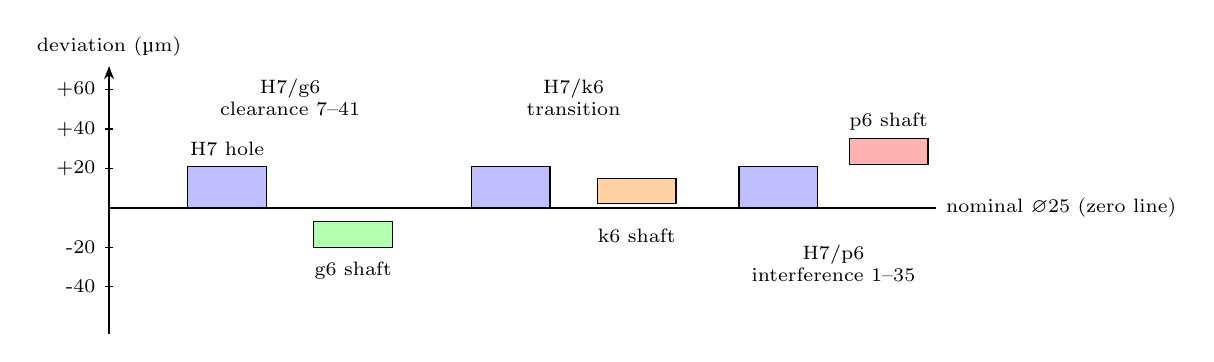
\begin{tikzpicture}[>=Stealth,font=\scriptsize,scale=1.0]
% zero line
\draw[thick] (0,0) -- (10.5,0) node[right] {nominal $\varnothing$25 (zero line)};
\draw[->] (0,-1.6) -- (0,1.8) node[above] {deviation (\si{\micro m})};
\foreach \y/\l in {0.5/+20,1.0/+40,1.5/+60,-0.5/-20,-1.0/-40} \draw (0.05,\y)--(-0.05,\y) node[left] {\l};
% hole H7: 0..+21 -> scale 40um = 1 unit -> 0.525
\fill[blue!25] (1.0,0) rectangle (2.0,0.525); \draw (1.0,0) rectangle (2.0,0.525); \node at (1.5,0.75) {H7 hole};
% shaft g6: -7..-20
\fill[green!30] (2.6,-0.5) rectangle (3.6,-0.175); \draw (2.6,-0.5) rectangle (3.6,-0.175); \node at (3.1,-0.8) {g6 shaft};
\node[align=center] at (2.3,1.4) {H7/g6\\ clearance 7--41};
% hole H7 again
\fill[blue!25] (4.6,0) rectangle (5.6,0.525); \draw (4.6,0) rectangle (5.6,0.525);
% shaft k6: +2..+15
\fill[orange!35] (6.2,0.05) rectangle (7.2,0.375); \draw (6.2,0.05) rectangle (7.2,0.375); \node at (6.7,-0.35) {k6 shaft};
\node[align=center] at (5.9,1.4) {H7/k6\\ transition};
% hole H7 again
\fill[blue!25] (8.0,0) rectangle (9.0,0.525); \draw (8.0,0) rectangle (9.0,0.525);
% shaft p6: +22..+35
\fill[red!30] (9.4,0.55) rectangle (10.4,0.875); \draw (9.4,0.55) rectangle (10.4,0.875); \node at (9.9,1.1) {p6 shaft};
\node[align=center] at (9.2,-0.7) {H7/p6\\ interference 1--35};
\end{tikzpicture}
\vspace{4pt}

\begin{columns}[T]
\column{0.5\textwidth}\footnotesize
\begin{itemize}
  \item IT7 at $\varnothing$25 = \SI{21}{\micro m}; IT6 = \SI{13}{\micro m}
  \item Hole-basis system (H hole, vary the shaft) is the default: reamers and gauges are for standard holes
  \item Bushing in lug: H7/p6 or s6 --- pressed, stays put, pre-stresses the lug (fatigue benefit)
\end{itemize}
\column{0.5\textwidth}\footnotesize
\begin{itemize}
  \item Pin in bushing: H7/g6 or f7 --- rotates, needs lubrication, hammering if clearance grows
  \item Bearing seats: shaft k6/m6, housing H7/J7 depending on which ring rotates
  \item A tolerance is a \emph{cost}: IT6 costs 2--3$\times$ IT9. Tolerance only what the function needs
\end{itemize}
\end{columns}
\end{frame}

\begin{frame}{Example: shaft drawing with GD\&T for a bearing seat}
\centering
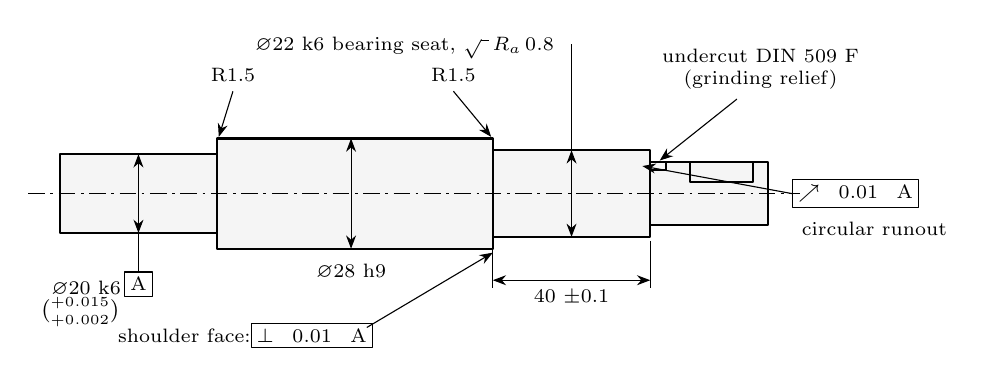
\begin{tikzpicture}[scale=1.0,>=Stealth,line join=round,font=\scriptsize]
% stepped shaft
\draw[thick,fill=gray!8] (0,-0.5) rectangle (2.0,0.5);
\draw[thick,fill=gray!8] (2.0,-0.7) rectangle (5.5,0.7);
\draw[thick,fill=gray!8] (5.5,-0.55) rectangle (7.5,0.55);
\draw[thick,fill=gray!8] (7.5,-0.4) rectangle (9.0,0.4);
% fillets marked
\draw[->] (2.2,1.3) -- (2.02,0.72); \node[anchor=south] at (2.2,1.3) {R1.5};
\draw[->] (5.0,1.3) -- (5.48,0.72); \node[anchor=south] at (5.0,1.3) {R1.5};
% undercut
\draw[thick] (7.5,0.4) -- (7.5,0.3) -- (7.7,0.3) -- (7.7,0.4);
\draw[->] (8.6,1.2) -- (7.62,0.42); \node[anchor=south,align=center] at (8.9,1.2) {undercut DIN 509 F\\ (grinding relief)};
% keyway on right end
\draw[thick] (8.0,0.4) rectangle (8.8,0.15);
% centreline
\draw[dash pattern=on 6pt off 2pt on 1pt off 2pt] (-0.4,0) -- (9.4,0);
% datum A on left journal
\draw (1.0,-0.5) -- (1.0,-1.0); \node[draw,inner sep=2pt] at (1.0,-1.15) {A};
% dims
\draw[<->] (1.0,-0.5) -- (1.0,0.5); \node[anchor=east,align=right] at (0.9,-1.4) {$\varnothing$20 k6\\ $\big(^{+0.015}_{+0.002}\big)$};
\draw[<->] (6.5,-0.55) -- (6.5,0.55); \draw (6.5,0.55) -- (6.5,1.9); \node[anchor=east,align=left] at (6.4,1.85) {$\varnothing$22 k6 bearing seat, $\sqrt{\ }\,R_a\,0.8$};
\node[draw,inner sep=2pt,anchor=west] at (9.3,0.0) {$\nearrow$ \, 0.01 \, A}; \node[anchor=west] at (9.3,-0.45) {circular runout}; \draw[->] (9.3,0) -- (7.4,0.35);
\draw[<->] (3.7,-0.7) -- (3.7,0.7); \node at (3.7,-1.0) {$\varnothing$28 h9};
\draw[<->] (5.5,-1.1) -- (7.5,-1.1) node[midway,below] {40 $\pm$0.1}; \draw (5.5,-0.6) -- (5.5,-1.2); \draw (7.5,-0.6) -- (7.5,-1.2);
% shoulder perpendicularity
\node[draw,inner sep=2pt] at (3.2,-1.8) {$\perp$ \, 0.01 \, A}; \draw[->] (3.9,-1.7) -- (5.5,-0.75);
\node[anchor=east] at (2.55,-1.8) {shoulder face:};
\end{tikzpicture}
\vspace{6pt}

\footnotesize Everything on this drawing exists because of a machine-element function: k6 so the inner ring does not creep, $R_a$ 0.8 so the seat does not fret, R1.5 fillets smaller than the bearing chamfer so the ring seats against a square shoulder, runout 0.01 so the bearing does not see a wobble, the undercut so the grinder can finish the seat to the shoulder.
\end{frame}

\begin{frame}{Standard parts: read the part number}
\footnotesize
\begin{tabular}{@{}ll@{}}
\toprule
Callout & Meaning \\
\midrule
NAS6204-10 & 1/4-28 UNJF close-tolerance shear bolt, 160 ksi, grip 10/16 in \\
MS21042-4 & 1/4-28 self-locking reduced hex nut \\
NAS1097AD4-5 & 1/8 in 2117 shear-head rivet, reduced head \\
AN960-416 & 1/4 in flat washer \\
MS14101-6 & Airframe spherical plain bearing, 3/8 in bore \\
NAS75-6 & Flanged press-fit bushing \\
\bottomrule
\end{tabular}
\vspace{6pt}

\begin{itemize}
  \item A standard part brings certified strength data with it (NASM1312 tests) --- you cite, you don't re-derive
  \item Mixing metric (ISO) and inch (NAS/MS) systems on one aircraft is a classic source of error; Turkish programmes increasingly use EN/ISO equivalents (EN 6114 etc.)
\end{itemize}
\end{frame}


\section{Standards: what they are, using bolts and nuts as the example}

\begin{frame}{Why standards exist, and who writes them}
\footnotesize
\begin{columns}[T]
\column{0.5\textwidth}
A standard fixes \alert{geometry, material, process, test method and acceptance} so that any supplier's part is interchangeable and its strength is known without testing it yourself.
\begin{itemize}
  \item \textbf{International}: ISO, IEC
  \item \textbf{Regional/national}: EN (CEN), DIN, BS, ASME, ASTM, TSE
  \item \textbf{Industry}: SAE (AS, AMS, ARP), AGMA, AWS
  \item \textbf{Aerospace parts}: NAS (AIA), MS/AN (US military, now NASM under SAE), LN (German aerospace), EN 6xxx/EN 2xxx (European aerospace)
  \item \textbf{Space}: ECSS (Europe), NASA-STD
  \item \textbf{Regulatory}: CS-25, FAR 25 --- these are \emph{law}, not standards
\end{itemize}
\column{0.5\textwidth}
\begin{block}{The hierarchy you will meet on a bolt}
\begin{itemize}
  \item Thread form: ISO 68 / ASME B1.1 / SAE AS8879
  \item Dimensions and grip: NAS6204 or EN 6114
  \item Material and heat treatment: AMS 6415 (4340), AMS 4928 (Ti-6Al-4V)
  \item Finish: AMS-QQ-P-416 (Cd), AMS 2451 (Zn--Ni)
  \item Test and qualification: NASM1312, ISO 898-1
  \item Installation: torque per MIL-HDBK-60 or NASA-STD-5020
\end{itemize}
\end{block}
\end{columns}
\end{frame}

\begin{frame}{Thread standards: metric ISO vs.\ unified UN/UNJ}
\footnotesize
\begin{columns}[T]
\column{0.5\textwidth}
\textbf{ISO metric} (ISO 68-1, 261, 262, 965)
\begin{itemize}
  \item Designation: M8$\times$1.25-6g (external), M8-6H (internal)
  \item 60$^\circ$ thread, coarse/fine pitch series
  \item Tolerance class: number = grade (4--8), letter = position (g, h external; H internal); 6g/6H is default
  \item Root radius optional $\Rightarrow$ poor fatigue unless ``MJ'' (ISO 5855, aerospace)
\end{itemize}
\column{0.5\textwidth}
\textbf{Unified inch} (ASME B1.1) and \textbf{UNJ} (SAE AS8879)
\begin{itemize}
  \item Designation: 1/4-28 UNF-3A (external), -3B (internal)
  \item UNC coarse, UNF fine, UNEF extra-fine; class 1A/2A/3A loosest to tightest
  \item \alert{UNJ}: mandatory rounded root radius 0.15--0.18$p$ $\Rightarrow$ $K_t$ from $\sim$3.8 down to $\sim$2.7; fatigue life 2--3$\times$
  \item All NAS/MS structural bolts are UNJF-3A; nuts UNJF-3B
\end{itemize}
\end{columns}
\vspace{4pt}
\begin{alertblock}{Aerospace rule}
Rolled (not cut) threads, rolled \emph{after} heat treatment, with J-root. A hardware-store M8 and an aerospace MJ8 bolt share a nominal size and differ 3$\times$ in fatigue life.
\end{alertblock}
\end{frame}


\begin{frame}{Anatomy of a structural bolt (NAS6204-type, hex head)}
\centering
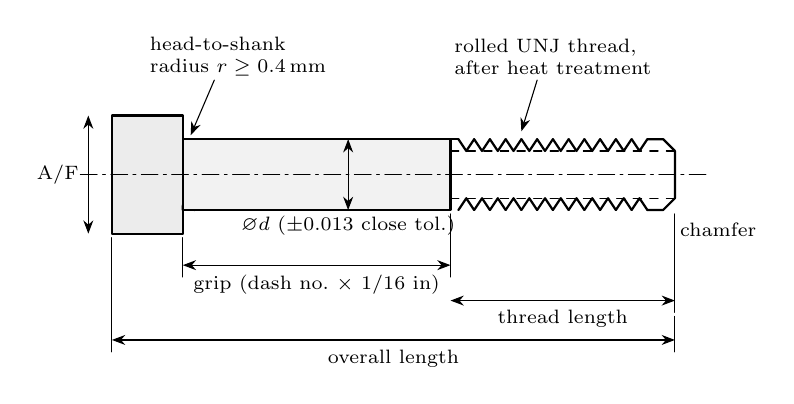
\begin{tikzpicture}[scale=1.0,>=Stealth,line cap=round,line join=round]
% head
\draw[thick,fill=gray!15] (0,-0.75) rectangle (0.9,0.75);
\draw (0,-0.75) -- (0,0.75);
% head to shank radius
\draw[thick,fill=gray!10] (0.9,-0.45) -- (0.9,-0.4) arc (180:90:0.15) -- (1.05,-0.45);
% shank (unthreaded)
\draw[thick,fill=gray!10] (0.9,-0.45) rectangle (4.3,0.45);
% thread region: zig-zag profile
\draw[thick] (4.3,0.45) -- (4.4,0.45);
\foreach \i in {0,...,11} {
  \draw[thick] ({4.4+\i*0.2},0.45) -- ({4.5+\i*0.2},0.3) -- ({4.6+\i*0.2},0.45);
  \draw[thick] ({4.4+\i*0.2},-0.45) -- ({4.5+\i*0.2},-0.3) -- ({4.6+\i*0.2},-0.45);
}
\draw[thick] (6.8,0.45) -- (7.0,0.45) -- (7.15,0.3) -- (7.15,-0.3) -- (7.0,-0.45) -- (6.8,-0.45);
% thread runout dashed
\draw[dashed] (4.3,-0.3) -- (7.15,-0.3); \draw[dashed] (4.3,0.3) -- (7.15,0.3);
% centreline
\draw[dash pattern=on 6pt off 2pt on 1pt off 2pt] (-0.4,0) -- (7.6,0);
% dimensions
\draw[<->] (0.9,-1.15) -- (4.3,-1.15) node[midway,below,font=\scriptsize] {grip (dash no.\ $\times$ 1/16 in)};
\draw (0.9,-0.8) -- (0.9,-1.3); \draw (4.3,-0.5) -- (4.3,-1.3);
\draw[<->] (4.3,-1.6) -- (7.15,-1.6) node[midway,below,font=\scriptsize] {thread length};
\draw (7.15,-0.5) -- (7.15,-1.75);
\draw[<->] (0,-2.1) -- (7.15,-2.1) node[midway,below,font=\scriptsize] {overall length};
\draw (0,-0.8) -- (0,-2.25); \draw (7.15,-1.8) -- (7.15,-2.25);
\draw[<->] (3.0,-0.45) -- (3.0,0.45); \node[font=\scriptsize] at (3.0,-0.65) {$\varnothing d$ ($\pm$0.013 close tol.)};
\draw[<->] (-0.3,-0.75) -- (-0.3,0.75) node[midway,left,font=\scriptsize] {A/F};
\node[font=\scriptsize,align=left] at (1.6,1.5) {head-to-shank\\ radius $r\ge 0.4$\,mm};
\draw[->] (1.3,1.2) -- (1.0,0.5);
\node[font=\scriptsize,align=left] at (5.6,1.5) {rolled UNJ thread,\\ after heat treatment};
\draw[->] (5.4,1.2) -- (5.2,0.55);
\node[font=\scriptsize] at (7.7,-0.7) {chamfer};
\end{tikzpicture}
\vspace{2pt}

\footnotesize Marking on head: manufacturer, material/strength symbol (e.g. triangle = 160 ksi, `T' = titanium). Head-to-shank fillet is the fatigue-critical location on the bolt after the first engaged thread.
\end{frame}

\begin{frame}{Thread profile: UN vs.\ UNJ (and ISO M vs.\ MJ)}
\centering
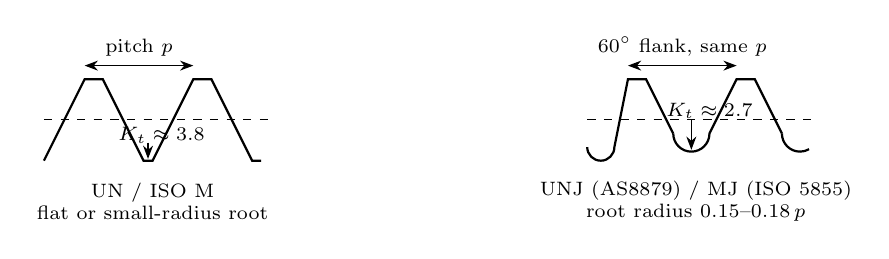
\begin{tikzpicture}[scale=1.15,>=Stealth]
% UN profile, sharp-ish root
\begin{scope}
\draw[thick] (0,0) -- (0.45,0.9) -- (0.65,0.9) -- (1.1,0) -- (1.2,0) -- (1.65,0.9) -- (1.85,0.9) -- (2.3,0) -- (2.4,0);
\draw[dashed] (0,0.45) -- (2.5,0.45);
\node[font=\scriptsize,align=center] at (1.2,-0.45) {UN / ISO M\\ flat or small-radius root};
\draw[<->] (0.45,1.05) -- (1.65,1.05) node[midway,above,font=\scriptsize] {pitch $p$};
\draw[->] (1.15,0.2) -- (1.15,0.02); \node[font=\scriptsize] at (1.3,0.28) {$K_t\approx3.8$};
\end{scope}
% UNJ profile with round root
\begin{scope}[xshift=6.0cm]
\draw[thick] (0,0.15) arc (180:360:0.15) -- (0.45,0.9) -- (0.65,0.9) -- (0.95,0.3);
\draw[thick] (0.95,0.3) arc (180:360:0.2) -- (1.65,0.9) -- (1.85,0.9) -- (2.15,0.3);
\draw[thick] (2.15,0.3) arc (180:300:0.2);
\draw[dashed] (0,0.45) -- (2.5,0.45);
\node[font=\scriptsize,align=center] at (1.2,-0.45) {UNJ (AS8879) / MJ (ISO 5855)\\ root radius $0.15$--$0.18\,p$};
\draw[->] (1.15,0.45) -- (1.15,0.12); \node[font=\scriptsize] at (1.35,0.55) {$K_t\approx2.7$};
\draw[<->] (0.45,1.05) -- (1.65,1.05) node[midway,above,font=\scriptsize] {60$^\circ$ flank, same $p$};
\end{scope}
\end{tikzpicture}
\vspace{6pt}

\begin{columns}[T]
\column{0.5\textwidth}\footnotesize
\begin{itemize}
  \item Same major/pitch diameter: a UNJ bolt fits a UN nut, but a UN bolt in a UNJ nut may not (larger minor diameter of the J-nut)
  \item Rolled thread: fibres follow the root, compressive residual stress $\Rightarrow$ fatigue life 2--3$\times$ over cut thread
\end{itemize}
\column{0.5\textwidth}\footnotesize
\begin{itemize}
  \item Tensile stress area $A_t=\frac{\pi}{4}\big(d-0.9382p\big)^2$ (ISO)
  \item First engaged thread carries $\sim$35\% of the load in a rigid nut: the other fatigue-critical spot
\end{itemize}
\end{columns}
\end{frame}

\begin{frame}{Bolt strength classes: ISO 898-1 vs.\ aerospace strength levels}
\footnotesize
\begin{columns}[T]
\column{0.5\textwidth}
\textbf{ISO 898-1 property class} $X.Y$
\begin{itemize}
  \item $X\times100$ = $F_{tu}$ (MPa), $X\times Y\times 10$ = $F_{ty}$
  \item 8.8: 800/640; 10.9: 1040/940; 12.9: 1220/1100
  \item Nuts: ISO 898-2 class 8, 10, 12 matched to bolt
  \item Ground machinery, some GA aircraft, ground support equipment
\end{itemize}
\column{0.5\textwidth}
\textbf{Aerospace strength levels (ksi / MPa)}
\begin{itemize}
  \item 95 ksi (655): low-strength Al or CRES bolts
  \item 125 ksi (860): AN bolts, 8740 steel --- older aircraft
  \item 160 ksi (1100): NAS6200 series, 4340/8740 --- current standard
  \item 180 ksi (1240): NAS1103--1120 high-strength steel
  \item 220 ksi (1520): NAS7xxx, H-11 / MP35N --- landing gear
  \item Ti-6Al-4V: 160 ksi, at 55\% of the mass of steel
\end{itemize}
\end{columns}
\vspace{4pt}
\small Standards give $F_{tu}$ and shear strength $F_{su}\approx 0.6F_{tu}$ (95 ksi shear for 160 ksi bolts) \emph{as a qualified value}: the allowable comes with the part number, and NASM1312 defines how it was tested (tension, double shear, fatigue, stress durability).
\end{frame}

\begin{frame}{Decoding a bolt: NAS6204-10 and EN 6114-4-10}
\footnotesize
\begin{columns}[T]
\column{0.5\textwidth}
\textbf{NAS6204-10}
\begin{itemize}
  \item NAS62\textbf{04}: 1/4 in nominal diameter (04 $\times$ 1/16 in), 1/4-28 UNJF-3A
  \item NAS620x series: close-tolerance shear bolt, 160 ksi, hex head, alloy steel, Cd plated
  \item -\textbf{10}: grip length 10/16 in = \SI{15.9}{mm} (unthreaded shank length)
  \item Suffix letters: D = drilled shank, H = drilled head, T = Ti alloy (NAS6204T10), C = CRES
  \item Shank diameter tolerance $\pm$\SI{0.013}{mm} (``close tolerance'') for use in reamed holes
\end{itemize}
\column{0.5\textwidth}
\textbf{EN 6114-4-10} (European metric equivalent)
\begin{itemize}
  \item EN 6114: hexagon-head, close-tolerance, MJ thread, Ti-6Al-4V, 1100 MPa class
  \item -\textbf{4}: code for MJ6$\times$1 thread, shank \SI{6}{mm}
  \item -\textbf{10}: grip code, in \SI{1}{mm} steps
  \item Companion nut: EN 6116 or LN 9161 (self-locking, MJ6)
\end{itemize}
\begin{block}{Grip is a design choice}
Threads must not be in the shear plane: grip $\ge$ stack-up, then one washer under the nut takes the rest.
\end{block}
\end{columns}
\end{frame}

\begin{frame}{Nut standards and locking}
\scriptsize
\begin{tabular}{@{}p{2.6cm}p{4.6cm}p{6.4cm}@{}}
\toprule
Standard & Type & Notes \\
\midrule
ISO 4032 / DIN 934 & Plain hex nut & Ground machinery only; needs a locking device \\
ISO 7040 / DIN 985 & Nylon-insert lock nut & Not above \SI{120}{\celsius}; single use \\
MS21042 & All-metal self-locking, reduced hex, 160 ksi & Standard structural nut; \SI{232}{\celsius} \\
MS21044 & Nylon-insert self-locking & \SI{121}{\celsius} limit; not for engine bays \\
MS21045 & All-metal, 180 ksi & High-strength bolts \\
MS17825 / AN310 & Castellated & With cotter pin; landing gear, control pins \\
NAS1291 & Miniature all-metal lock nut & Ti or CRES; weight-critical \\
EN 6116, LN 9161 & Metric self-locking, MJ thread & European programmes \\
\bottomrule
\end{tabular}
\vspace{4pt}
\begin{itemize}
  \item CS-25.607: no self-locking nut on any bolt subject to rotation in operation unless a non-friction locking device is added; self-locking nuts must meet AS3350 (torque retention after 15 cycles)
  \item Lockwire (MS33540), safety cable, cotter pin, tab washer --- ``positive'' locking for anything that can back off and hurt someone
\end{itemize}
\end{frame}


\begin{frame}{Nut cross-sections: plain, all-metal self-locking, castellated}
\centering
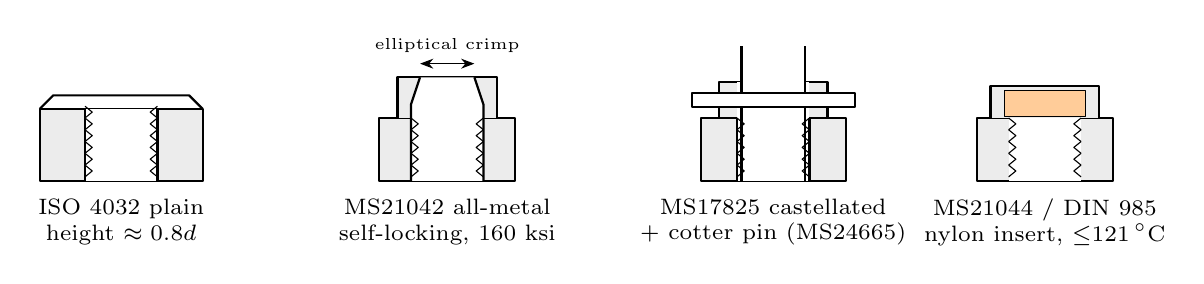
\begin{tikzpicture}[scale=1.15,>=Stealth,line join=round,every node/.style={transform shape}]
% plain hex nut section
\begin{scope}
\draw[thick,fill=gray!15] (-0.9,0) rectangle (0.9,0.8);
\fill[white] (-0.4,0) rectangle (0.4,0.8);
\foreach \i in {0,...,5} {\draw ( -0.4,{0.05+\i*0.13}) -- (-0.32,{0.115+\i*0.13}) -- (-0.4,{0.18+\i*0.13}); \draw (0.4,{0.05+\i*0.13}) -- (0.32,{0.115+\i*0.13}) -- (0.4,{0.18+\i*0.13});}
\draw[thick] (-0.4,0) -- (-0.4,0.8) (0.4,0) -- (0.4,0.8);
\draw[thick] (-0.9,0.8) -- (-0.75,0.95) -- (0.75,0.95) -- (0.9,0.8);
\node[font=\scriptsize,align=center] at (0,-0.45) {ISO 4032 plain\\ height $\approx0.8d$};
\end{scope}
% all-metal self-locking (MS21042): reduced hex, elliptical crimp at top
\begin{scope}[xshift=3.6cm]
\draw[thick,fill=gray!15] (-0.75,0) rectangle (0.75,0.7);
\draw[thick,fill=gray!15] (-0.55,0.7) -- (-0.55,1.15) -- (0.55,1.15) -- (0.55,0.7);
\fill[white] (-0.4,0) rectangle (0.4,0.7);
\fill[white] (-0.4,0.7) -- (-0.4,0.85) -- (-0.3,1.15) -- (0.3,1.15) -- (0.4,0.85) -- (0.4,0.7);
\foreach \i in {0,...,4} {\draw (-0.4,{0.05+\i*0.13}) -- (-0.32,{0.115+\i*0.13}) -- (-0.4,{0.18+\i*0.13}); \draw (0.4,{0.05+\i*0.13}) -- (0.32,{0.115+\i*0.13}) -- (0.4,{0.18+\i*0.13});}
\draw[thick] (-0.4,0) -- (-0.4,0.85) -- (-0.3,1.15) (0.4,0) -- (0.4,0.85) -- (0.3,1.15);
\draw[<->] (-0.3,1.3) -- (0.3,1.3) node[midway,above,font=\tiny] {elliptical crimp};
\node[font=\scriptsize,align=center] at (0,-0.45) {MS21042 all-metal\\ self-locking, 160 ksi};
\end{scope}
% castellated nut with cotter pin
\begin{scope}[xshift=7.2cm]
\draw[thick,fill=gray!15] (-0.8,0) rectangle (0.8,0.7);
\draw[thick,fill=gray!15] (-0.6,0.7) rectangle (-0.35,1.1);
\draw[thick,fill=gray!15] (0.35,0.7) rectangle (0.6,1.1);
\fill[white] (-0.4,0) rectangle (0.4,1.1);
\foreach \i in {0,...,4} {\draw (-0.4,{0.05+\i*0.13}) -- (-0.32,{0.115+\i*0.13}) -- (-0.4,{0.18+\i*0.13}); \draw (0.4,{0.05+\i*0.13}) -- (0.32,{0.115+\i*0.13}) -- (0.4,{0.18+\i*0.13});}
\draw[thick] (-0.4,0) -- (-0.4,0.7) (0.4,0) -- (0.4,0.7);
% bolt shank with cross hole and cotter pin
\draw[thick] (-0.35,0) -- (-0.35,1.5) (0.35,0) -- (0.35,1.5);
\draw[thick,fill=white] (-0.9,0.82) rectangle (0.9,0.98);
\node[font=\scriptsize,align=center] at (0,-0.45) {MS17825 castellated\\ + cotter pin (MS24665)};
\end{scope}
% nylon insert
\begin{scope}[xshift=10.2cm]
\draw[thick,fill=gray!15] (-0.75,0) rectangle (0.75,0.7);
\draw[thick,fill=gray!15] (-0.6,0.7) -- (-0.6,1.05) -- (0.6,1.05) -- (0.6,0.7);
\fill[white] (-0.4,0) rectangle (0.4,0.7);
\fill[orange!40] (-0.45,0.72) rectangle (0.45,1.0);
\draw (-0.45,0.72) rectangle (0.45,1.0);
\foreach \i in {0,...,4} {\draw (-0.4,{0.05+\i*0.13}) -- (-0.32,{0.115+\i*0.13}) -- (-0.4,{0.18+\i*0.13}); \draw (0.4,{0.05+\i*0.13}) -- (0.32,{0.115+\i*0.13}) -- (0.4,{0.18+\i*0.13});}
\node[font=\scriptsize,align=center] at (0,-0.45) {MS21044 / DIN 985\\ nylon insert, $\le$\SI{121}{\celsius}};
\end{scope}
\end{tikzpicture}
\vspace{6pt}

\footnotesize All-metal self-locking nuts get their prevailing torque from a deformed (out-of-round) top; AS3350 requires the torque to survive 15 install/remove cycles. Castellated + cotter pin is the only positive lock accepted for rotating pins (CS-25.607). Nylon-insert nuts are excluded from hot zones and from primary structure on most programmes.
\end{frame}

\begin{frame}{The joint: grip, washers and the shear plane}
\centering
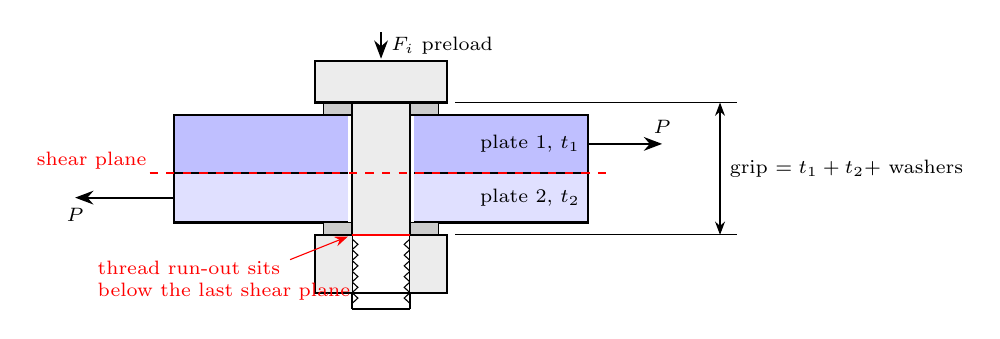
\begin{tikzpicture}[scale=1.05,>=Stealth]
% plates
\fill[blue!12] (0,0) rectangle (5,0.6);
\fill[blue!25] (0,0.6) rectangle (5,1.3);
\draw[thick] (0,0) rectangle (5,0.6); \draw[thick] (0,0.6) rectangle (5,1.3);
\node[font=\scriptsize] at (4.3,0.3) {plate 2, $t_2$}; \node[font=\scriptsize] at (4.3,0.95) {plate 1, $t_1$};
% hole
\fill[white] (2.1,0) rectangle (2.9,1.3);
% washer under head
\fill[gray!40] (1.8,1.3) rectangle (3.2,1.45); \draw (1.8,1.3) rectangle (3.2,1.45);
% washer under nut
\fill[gray!40] (1.8,-0.15) rectangle (3.2,0); \draw (1.8,-0.15) rectangle (3.2,0);
% bolt
\fill[gray!15] (2.15,-0.15) rectangle (2.85,1.45); \draw[thick] (2.15,-0.15) -- (2.15,1.45) (2.85,-0.15) -- (2.85,1.45);
\fill[gray!15] (1.7,1.45) rectangle (3.3,1.95); \draw[thick] (1.7,1.45) rectangle (3.3,1.95);
% thread below
\foreach \i in {0,...,5} {\draw (2.15,{-0.2-\i*0.13}) -- (2.22,{-0.265-\i*0.13}) -- (2.15,{-0.33-\i*0.13}); \draw (2.85,{-0.2-\i*0.13}) -- (2.78,{-0.265-\i*0.13}) -- (2.85,{-0.33-\i*0.13});}
\draw[thick] (2.15,-0.15) -- (2.15,-1.05) (2.85,-0.15) -- (2.85,-1.05) (2.15,-1.05) -- (2.85,-1.05);
% nut
\fill[gray!15] (1.7,-0.15) rectangle (2.15,-0.85); \fill[gray!15] (2.85,-0.15) rectangle (3.3,-0.85);
\draw[thick] (1.7,-0.15) rectangle (3.3,-0.85);
% thread runout mark
\draw[red,thick] (2.15,-0.15) -- (2.85,-0.15);
\node[red,font=\scriptsize,align=left] at (0.6,-0.7) {thread run-out sits\\ below the last shear plane};
\draw[->,red] (1.4,-0.45) -- (2.1,-0.17);
% shear plane
\draw[dashed,red,thick] (-0.3,0.6) -- (5.3,0.6); \node[red,font=\scriptsize] at (-1.0,0.75) {shear plane};
% loads
\draw[->,thick] (5,0.95) -- (5.9,0.95) node[above,font=\scriptsize] {$P$};
\draw[->,thick] (0,0.3) -- (-1.2,0.3) node[below,font=\scriptsize] {$P$};
% grip dimension
\draw[<->] (6.6,-0.15) -- (6.6,1.45) node[midway,right,font=\scriptsize] {grip $= t_1+t_2+$ washers};
\draw (3.4,-0.15) -- (6.8,-0.15); \draw (3.4,1.45) -- (6.8,1.45);
% preload
\draw[->,thick] (2.5,2.3) -- (2.5,1.98) node[midway,right,font=\scriptsize] {$F_i$ preload};
\end{tikzpicture}
\vspace{4pt}

\footnotesize Choose grip $\ge$ stack-up so the unthreaded shank spans every shear plane; take up the excess with at most two washers under the nut. A thread in the shear plane halves shear area and puts $K_t$ where the load is.
\end{frame}

\begin{frame}{Washers, holes and the joint as a system}
\footnotesize
\begin{columns}[T]
\column{0.5\textwidth}
\begin{itemize}
  \item Washers: AN960 (plain, Cd steel), NAS1149 (metric/inch, various materials), countersunk washers under the head of a bolt with a head-to-shank radius
  \item Hole: reamed to H7-class for close-tolerance bolts; clearance \SI{0.05}{}--\SI{0.1}{mm} for standard bolts; interference (\SI{0.02}{}--\SI{0.05}{mm}) with taper-lok / Hi-Lok for fatigue
  \item Countersinks per NAS or EN 4xxx, depth $\le 0.7t$ (knife edge otherwise)
\end{itemize}
\column{0.5\textwidth}
\begin{block}{Reading a standard: what to look for}
\begin{enumerate}
  \item Scope --- does it cover my size/material/temperature?
  \item Dimensions and tolerances table
  \item Material, heat treatment, finish references
  \item Mechanical properties: tensile, double shear, fatigue, stress durability
  \item Qualification and lot acceptance tests
  \item Marking --- how to verify what is in your hand
\end{enumerate}
\end{block}
\end{columns}
\vspace{4pt}
\small The mechanics (thread stress, preload, torque--tension) and the joint analysis come later. Today: you can read the callout and know what it promises.
\end{frame}

\section{Design principles and typical errors}

\begin{frame}{Eight principles that survive every textbook}
\begin{enumerate}
  \item \alert{Direct load path}: force goes straight from A to B; every offset is a bending moment
  \item \alert{Fasteners in shear, not bending}: a bolt is a pin, not a beam
  \item \alert{Stiffness compatibility}: load follows stiffness; a stiff element next to a soft one takes everything
  \item \alert{No sharp corners}: radius everything; $K_t$ is where fatigue starts
  \item \alert{Symmetry}: avoid eccentric single-shear joints where you can
  \item \alert{Self-help}: let the load tighten, not loosen, the joint (preload, taper, direction of thread)
  \item \alert{Inspectability and replaceability}: if it cannot be inspected, it must be safe-life with a big factor
  \item \alert{Fail-safe or damage-tolerant}: a second load path, or a crack that is found before it is critical
\end{enumerate}
\end{frame}

\begin{frame}{A gallery of common errors (you will see each of these again)}
\scriptsize
\begin{tabular}{@{}p{6.2cm}p{7cm}@{}}
\toprule
Error & Consequence \\
\midrule
Sharp internal corner, no radius on fillet & Fatigue crack at $K_t\approx 3$ \\
Bolt loaded in bending by a misaligned clevis & Bolt fatigue, hole ovalisation \\
Unspecified preload / no torque note & Joint slips, fretting, bolt fatigue \\
Thin flange, thick web (stiffness jump) & Load piles into first fastener row \\
Tolerance stack-up ignored across an assembly & Bearings pre-loaded to death or loose \\
Weld toe left as-welded at a stressed edge & Weld fatigue class collapses \\
Dissimilar metals without isolation & Galvanic corrosion, hidden section loss \\
Pocket that traps water & Crevice corrosion, SCC \\
Thread run-out in the shear plane & Reduced area, $K_t$ at the worst place \\
Single load path with no inspection access & Safe-life with no margin for error \\
\bottomrule
\end{tabular}
\end{frame}


\begin{frame}{Errors 1--2: sharp internal corner; bolt loaded in bending}
\centering
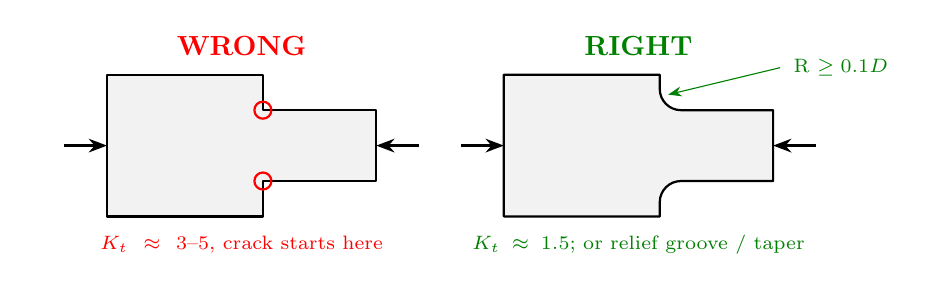
\begin{tikzpicture}[scale=0.9,>=Stealth,line join=round,font=\scriptsize]
% --- 1 wrong: stepped bar with sharp corner
\begin{scope}
\draw[thick,fill=gray!10] (0,0) -- (2.2,0) -- (2.2,0.5) -- (3.8,0.5) -- (3.8,1.5) -- (2.2,1.5) -- (2.2,2.0) -- (0,2.0) -- cycle;
\draw[red,thick] (2.2,0.5) circle (0.12); \draw[red,thick] (2.2,1.5) circle (0.12);
\draw[->,thick] (-0.6,1.0) -- (0,1.0); \draw[->,thick] (4.4,1.0) -- (3.8,1.0);
\node[red,capt] at (1.9,-0.4) {$K_t\approx 3$--5, crack starts here};
\node[red,font=\bfseries] at (1.9,2.4) {WRONG};
\end{scope}
\begin{scope}[xshift=5.6cm]
\draw[thick,fill=gray!10] (0,0) -- (2.2,0) -- (2.2,0.2) arc (180:90:0.3) -- (3.8,0.5) -- (3.8,1.5) -- (2.5,1.5) arc (270:180:0.3) -- (2.2,2.0) -- (0,2.0) -- cycle;
\draw[->,thick] (-0.6,1.0) -- (0,1.0); \draw[->,thick] (4.4,1.0) -- (3.8,1.0);
\draw[->,green!50!black] (3.9,2.1) -- (2.32,1.72); \node[green!50!black,anchor=west] at (3.95,2.1) {R $\ge 0.1D$};
\node[green!50!black,capt] at (1.9,-0.4) {$K_t\approx 1.5$; or relief groove / taper};
\node[green!50!black,font=\bfseries] at (1.9,2.4) {RIGHT};
\end{scope}
\end{tikzpicture}

\vspace{2pt}
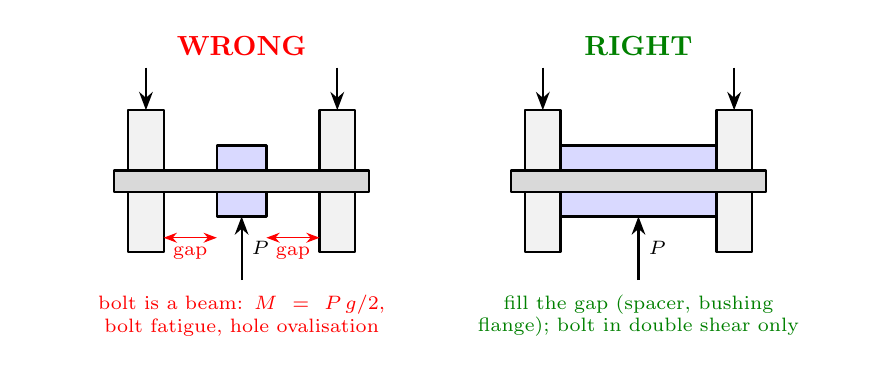
\begin{tikzpicture}[scale=0.9,>=Stealth,line join=round,font=\scriptsize]
% --- 2 wrong: clevis with big gap, bolt bends
\begin{scope}
\draw[thick,fill=gray!10] (0,0) rectangle (0.5,2.0); \draw[thick,fill=gray!10] (2.7,0) rectangle (3.2,2.0);
\draw[thick,fill=blue!15] (1.25,0.5) rectangle (1.95,1.5);
\draw[thick,fill=gray!30] (-0.2,0.85) rectangle (3.4,1.15);
\draw[->,thick] (1.6,-0.4) -- (1.6,0.5) node[midway,right] {$P$};
\draw[->,thick] (0.25,2.6) -- (0.25,2.0); \draw[->,thick] (2.95,2.6) -- (2.95,2.0);
\draw[red,<->] (0.5,0.2) -- (1.25,0.2) node[midway,below] {gap};
\draw[red,<->] (1.95,0.2) -- (2.7,0.2) node[midway,below] {gap};
\node[red,capt] at (1.6,-0.9) {bolt is a beam: $M = P\,g/2$, bolt fatigue, hole ovalisation};
\node[red,font=\bfseries] at (1.6,2.9) {WRONG};
\end{scope}
\begin{scope}[xshift=5.6cm]
\draw[thick,fill=gray!10] (0,0) rectangle (0.5,2.0); \draw[thick,fill=gray!10] (2.7,0) rectangle (3.2,2.0);
\draw[thick,fill=blue!15] (0.5,0.5) rectangle (2.7,1.5);
\draw[thick,fill=gray!30] (-0.2,0.85) rectangle (3.4,1.15);
\draw[->,thick] (1.6,-0.4) -- (1.6,0.5) node[midway,right] {$P$};
\draw[->,thick] (0.25,2.6) -- (0.25,2.0); \draw[->,thick] (2.95,2.6) -- (2.95,2.0);
\node[green!50!black,capt] at (1.6,-0.9) {fill the gap (spacer, bushing flange); bolt in double shear only};
\node[green!50!black,font=\bfseries] at (1.6,2.9) {RIGHT};
\end{scope}
\end{tikzpicture}
\end{frame}

\begin{frame}{Errors 3--4: preload not specified; stiffness jump at a splice}
\centering
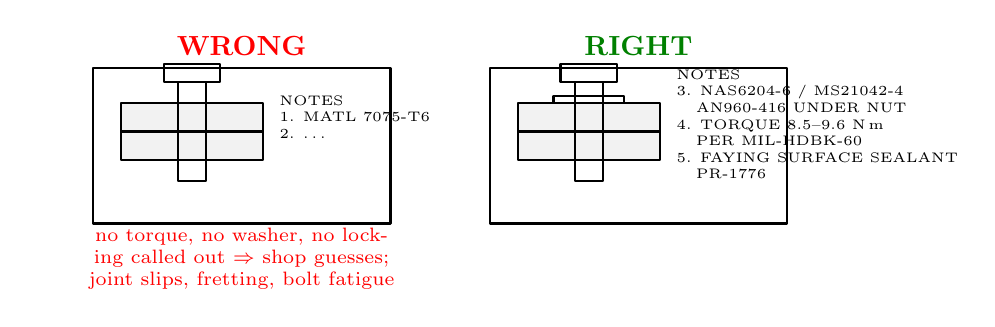
\begin{tikzpicture}[scale=0.9,>=Stealth,line join=round,font=\scriptsize]
% --- 3: drawing snippet, note missing vs present
\begin{scope}
\draw[thick] (0,0) rectangle (4.2,2.2);
\draw[thick,fill=gray!10] (0.4,0.9) rectangle (2.4,1.3); \draw[thick,fill=gray!10] (0.4,1.3) rectangle (2.4,1.7);
\draw[thick] (1.2,0.6) rectangle (1.6,2.0); \draw[thick] (1.0,2.0) rectangle (1.8,2.25);
\node[anchor=west,font=\tiny,align=left] at (2.5,1.5) {NOTES\\ 1. MATL 7075-T6\\ 2. \ldots};
\node[red,capt] at (2.1,-0.5) {no torque, no washer, no locking called out $\Rightarrow$ shop guesses; joint slips, fretting, bolt fatigue};
\node[red,font=\bfseries] at (2.1,2.5) {WRONG};
\end{scope}
\begin{scope}[xshift=5.6cm]
\draw[thick] (0,0) rectangle (4.2,2.2);
\draw[thick,fill=gray!10] (0.4,0.9) rectangle (2.4,1.3); \draw[thick,fill=gray!10] (0.4,1.3) rectangle (2.4,1.7);
\draw[thick] (1.2,0.6) rectangle (1.6,2.0); \draw[thick] (1.0,2.0) rectangle (1.8,2.25); \draw[thick] (0.9,1.7) rectangle (1.9,1.8);
\node[anchor=west,font=\tiny,align=left] at (2.5,1.4) {NOTES\\ 3. NAS6204-6 / MS21042-4\\ \ \ \ AN960-416 UNDER NUT\\ 4. TORQUE 8.5--9.6 N\,m\\ \ \ \ PER MIL-HDBK-60\\ 5. FAYING SURFACE SEALANT\\ \ \ \ PR-1776};
\node[green!50!black,font=\bfseries] at (2.1,2.5) {RIGHT};
\end{scope}
\end{tikzpicture}

\vspace{2pt}
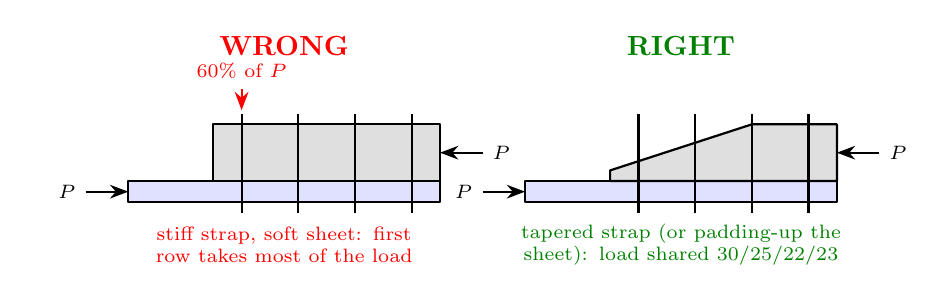
\begin{tikzpicture}[scale=0.9,>=Stealth,line join=round,font=\scriptsize]
% --- 4 wrong: thick strap onto thin sheet, abrupt
\begin{scope}
\draw[thick,fill=blue!12] (0,0) rectangle (4.4,0.3);
\draw[thick,fill=gray!25] (1.2,0.3) rectangle (4.4,1.1);
\foreach \x in {1.6,2.4,3.2,4.0} \draw[thick] (\x,-0.15) -- (\x,1.25);
\draw[->,thick] (-0.6,0.15) -- (0,0.15) node[pos=0,left] {$P$}; \draw[->,thick] (5.0,0.7) -- (4.4,0.7) node[pos=0,right] {$P$};
\draw[red,->,thick] (1.6,1.6) -- (1.6,1.3); \node[red,capt] at (1.6,1.85) {60\% of $P$};
\node[red,capt] at (2.2,-0.6) {stiff strap, soft sheet: first row takes most of the load};
\node[red,font=\bfseries] at (2.2,2.2) {WRONG};
\end{scope}
\begin{scope}[xshift=5.6cm]
\draw[thick,fill=blue!12] (0,0) rectangle (4.4,0.3);
\draw[thick,fill=gray!25] (1.2,0.3) -- (4.4,0.3) -- (4.4,1.1) -- (3.2,1.1) -- (1.2,0.45) -- cycle;
\foreach \x in {1.6,2.4,3.2,4.0} \draw[thick] (\x,-0.15) -- (\x,1.25);
\draw[->,thick] (-0.6,0.15) -- (0,0.15) node[pos=0,left] {$P$}; \draw[->,thick] (5.0,0.7) -- (4.4,0.7) node[pos=0,right] {$P$};
\node[green!50!black,capt] at (2.2,-0.6) {tapered strap (or padding-up the sheet): load shared 30/25/22/23};
\node[green!50!black,font=\bfseries] at (2.2,2.2) {RIGHT};
\end{scope}
\end{tikzpicture}
\end{frame}

\begin{frame}{Errors 5--6: over-constrained bearings; weld toe at a stressed edge}
\centering
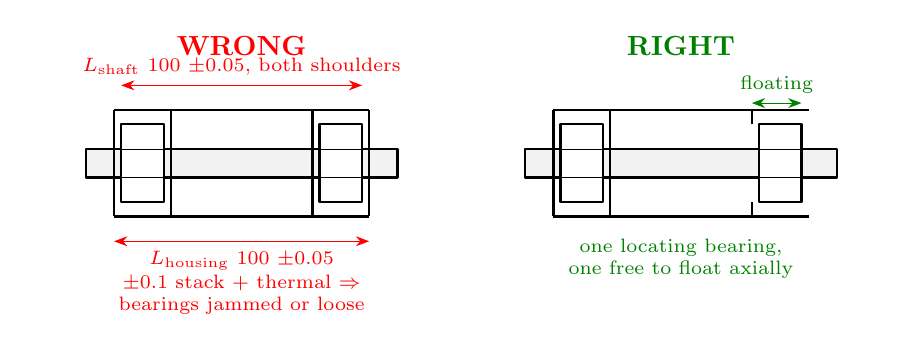
\begin{tikzpicture}[scale=0.9,>=Stealth,line join=round,font=\scriptsize]
% --- 5 wrong: shaft with two bearings both fixed axially
\begin{scope}
\draw[thick,fill=gray!10] (0,0.55) rectangle (4.4,0.95);
\foreach \x in {0.8,3.6} {\draw[thick,fill=white] (\x-0.3,0.2) rectangle (\x+0.3,1.3); \draw (\x-0.3,0.55) -- (\x+0.3,0.55) (\x-0.3,0.95) -- (\x+0.3,0.95); \draw[thick] (\x-0.4,0) -- (\x-0.4,1.5) (\x+0.4,0) -- (\x+0.4,1.5);}
\draw[thick] (0.4,1.5) -- (4.0,1.5); \draw[thick] (0.4,0) -- (4.0,0);
\draw[red,<->] (0.4,-0.35) -- (4.0,-0.35) node[midway,below] {$L_{\text{housing}}$ 100 $\pm$0.05};
\draw[red,<->] (0.5,1.85) -- (3.9,1.85) node[midway,above] {$L_{\text{shaft}}$ 100 $\pm$0.05, both shoulders};
\node[red,capt] at (2.2,-1.1) {$\pm$0.1 stack $+$ thermal $\Rightarrow$ bearings jammed or loose};
\node[red,font=\bfseries] at (2.2,2.4) {WRONG};
\end{scope}
\begin{scope}[xshift=6.2cm]
\draw[thick,fill=gray!10] (0,0.55) rectangle (4.4,0.95);
\foreach \x in {0.8,3.6} {\draw[thick,fill=white] (\x-0.3,0.2) rectangle (\x+0.3,1.3); \draw (\x-0.3,0.55) -- (\x+0.3,0.55) (\x-0.3,0.95) -- (\x+0.3,0.95);}
\draw[thick] (0.4,0) -- (0.4,1.5) (1.2,0) -- (1.2,1.5);
\draw[thick] (3.2,0) -- (3.2,0.2) (3.2,1.3) -- (3.2,1.5);
\draw[green!50!black,<->] (3.2,1.6) -- (3.9,1.6) node[midway,above] {floating};
\draw[thick] (0.4,1.5) -- (4.0,1.5); \draw[thick] (0.4,0) -- (4.0,0);
\node[green!50!black,capt] at (2.2,-0.6) {one locating bearing, one free to float axially};
\node[green!50!black,font=\bfseries] at (2.2,2.4) {RIGHT};
\end{scope}
\end{tikzpicture}

\vspace{2pt}
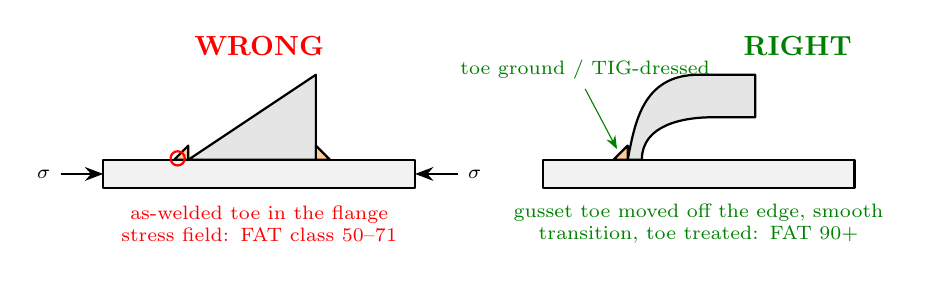
\begin{tikzpicture}[scale=0.9,>=Stealth,line join=round,font=\scriptsize]
% --- 6 wrong: gusset welded up to the flange edge, toe at max stress
\begin{scope}
\draw[thick,fill=gray!10] (0,0) rectangle (4.4,0.4);  % beam flange
\draw[thick,fill=gray!20] (1.2,0.4) -- (3.0,0.4) -- (3.0,1.6) -- cycle; % gusset
\draw[thick,fill=orange!40] (1.0,0.4) -- (1.2,0.4) -- (1.2,0.6) -- cycle; \draw[thick,fill=orange!40] (3.0,0.4) -- (3.2,0.4) -- (3.0,0.6) -- cycle;
\draw[red,thick] (1.05,0.42) circle (0.1);
\draw[->,thick] (-0.6,0.2) -- (0,0.2) node[pos=0,left] {$\sigma$}; \draw[->,thick] (5.0,0.2) -- (4.4,0.2) node[pos=0,right] {$\sigma$};
\node[red,capt] at (2.2,-0.5) {as-welded toe in the flange stress field: FAT class 50--71};
\node[red,font=\bfseries] at (2.2,2.0) {WRONG};
\end{scope}
\begin{scope}[xshift=6.2cm]
\draw[thick,fill=gray!10] (0,0) rectangle (4.4,0.4);
\draw[thick,fill=gray!20] (1.4,0.4) .. controls (1.4,0.9) and (2.0,1.0) .. (2.4,1.0) -- (3.0,1.0) -- (3.0,1.6) -- (2.2,1.6) .. controls (1.4,1.6) and (1.3,0.9) .. (1.2,0.4) -- cycle;
\draw[thick,fill=orange!40] (1.0,0.4) -- (1.2,0.4) -- (1.2,0.6) -- cycle;
\draw[green!50!black,->] (0.6,1.4) -- (1.05,0.55); \node[green!50!black,anchor=south] at (0.6,1.4) {toe ground / TIG-dressed};
\node[green!50!black,capt] at (2.2,-0.5) {gusset toe moved off the edge, smooth transition, toe treated: FAT 90+};
\node[green!50!black,font=\bfseries] at (3.6,2.0) {RIGHT};
\end{scope}
\end{tikzpicture}
\end{frame}

\begin{frame}{Errors 7--8: dissimilar metals in contact; a pocket that traps water}
\centering
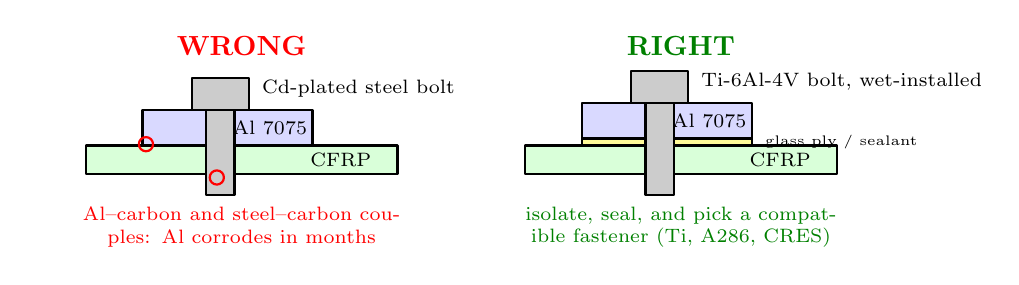
\begin{tikzpicture}[scale=0.9,>=Stealth,line join=round,font=\scriptsize]
% --- 7 wrong: Al bracket bolted to CFRP with steel bolt, no isolation
\begin{scope}
\draw[thick,fill=green!15] (0,0) rectangle (4.4,0.4); \node at (3.6,0.2) {CFRP};
\draw[thick,fill=blue!15] (0.8,0.4) rectangle (3.2,0.9); \node at (2.6,0.65) {Al 7075};
\draw[thick,fill=gray!40] (1.7,-0.3) rectangle (2.1,1.35); \draw[thick,fill=gray!40] (1.5,0.9) rectangle (2.3,1.35);
\node[anchor=west] at (2.35,1.2) {Cd-plated steel bolt};
\draw[red,thick] (0.85,0.42) circle (0.1); \draw[red,thick] (1.85,-0.05) circle (0.1);
\node[red,capt] at (2.2,-0.75) {Al--carbon and steel--carbon couples: Al corrodes in months};
\node[red,font=\bfseries] at (2.2,1.8) {WRONG};
\end{scope}
\begin{scope}[xshift=6.2cm]
\draw[thick,fill=green!15] (0,0) rectangle (4.4,0.4); \node at (3.6,0.2) {CFRP};
\draw[thick,fill=yellow!40] (0.8,0.4) rectangle (3.2,0.5); \node[anchor=west,font=\tiny] at (3.25,0.45) {glass ply / sealant};
\draw[thick,fill=blue!15] (0.8,0.5) rectangle (3.2,1.0); \node at (2.6,0.75) {Al 7075};
\draw[thick,fill=gray!40] (1.7,-0.3) rectangle (2.1,1.45); \draw[thick,fill=gray!40] (1.5,1.0) rectangle (2.3,1.45);
\node[anchor=west] at (2.35,1.3) {Ti-6Al-4V bolt, wet-installed};
\node[green!50!black,capt] at (2.2,-0.75) {isolate, seal, and pick a compatible fastener (Ti, A286, CRES)};
\node[green!50!black,font=\bfseries] at (2.2,1.8) {RIGHT};
\end{scope}
\end{tikzpicture}

\vspace{2pt}
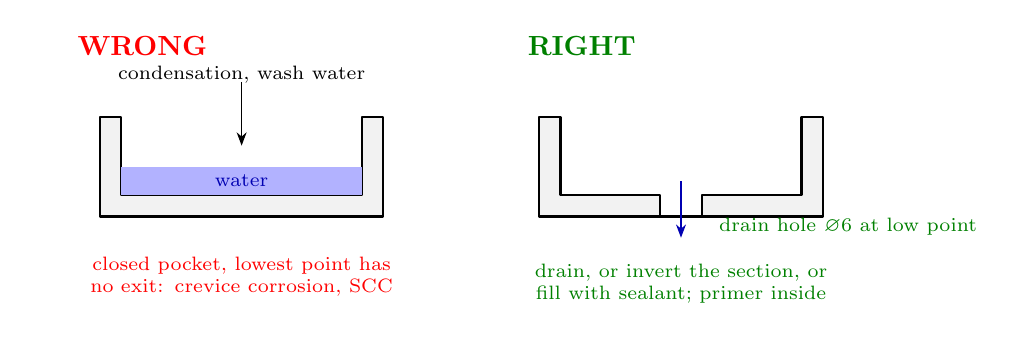
\begin{tikzpicture}[scale=0.9,>=Stealth,line join=round,font=\scriptsize]
% --- 8 wrong: channel section open upward
\begin{scope}
\draw[thick,fill=gray!10] (0,0) -- (0,1.4) -- (0.3,1.4) -- (0.3,0.3) -- (3.7,0.3) -- (3.7,1.4) -- (4.0,1.4) -- (4.0,0) -- cycle;
\fill[blue!30] (0.3,0.3) rectangle (3.7,0.7); \node[blue!70!black] at (2.0,0.5) {water};
\draw[->] (2.0,1.9) -- (2.0,1.0); \node at (2.0,2.0) {condensation, wash water};
\node[red,capt] at (2.0,-0.85) {closed pocket, lowest point has no exit: crevice corrosion, SCC};
\node[red,font=\bfseries] at (0.6,2.4) {WRONG};
\end{scope}
\begin{scope}[xshift=6.2cm]
\draw[thick,fill=gray!10] (0,0) -- (0,1.4) -- (0.3,1.4) -- (0.3,0.3) -- (1.7,0.3) -- (1.7,0) -- (2.3,0) -- (2.3,0.3) -- (3.7,0.3) -- (3.7,1.4) -- (4.0,1.4) -- (4.0,0) -- cycle;
\draw[->,blue!70!black] (2.0,0.5) -- (2.0,-0.3);
\node[green!50!black,anchor=west] at (2.4,-0.15) {drain hole $\varnothing$6 at low point};
\node[green!50!black,capt] at (2.0,-0.95) {drain, or invert the section, or fill with sealant; primer inside};
\node[green!50!black,font=\bfseries] at (0.6,2.4) {RIGHT};
\end{scope}
\end{tikzpicture}
\end{frame}

\begin{frame}{Errors 9--10: thread in the shear plane; single load path with no inspection access}
\centering
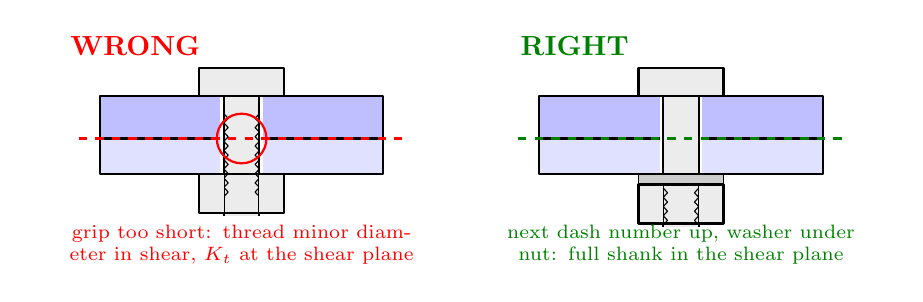
\begin{tikzpicture}[scale=0.9,>=Stealth,line join=round,font=\scriptsize]
% --- 9 wrong: too-short grip, thread in shear plane
\begin{scope}
\fill[blue!12] (0,0) rectangle (4.0,0.5); \fill[blue!25] (0,0.5) rectangle (4.0,1.1);
\draw[thick] (0,0) rectangle (4.0,0.5); \draw[thick] (0,0.5) rectangle (4.0,1.1);
\fill[white] (1.7,0) rectangle (2.3,1.1);
\fill[gray!15] (1.75,-0.6) rectangle (2.25,1.1); \draw[thick] (1.75,-0.6) -- (1.75,1.1) (2.25,-0.6) -- (2.25,1.1);
\fill[gray!15] (1.4,1.1) rectangle (2.6,1.5); \draw[thick] (1.4,1.1) rectangle (2.6,1.5);
\foreach \i in {0,...,8} {\draw (1.75,{0.85-\i*0.13}) -- (1.81,{0.785-\i*0.13}) -- (1.75,{0.72-\i*0.13}); \draw (2.25,{0.85-\i*0.13}) -- (2.19,{0.785-\i*0.13}) -- (2.25,{0.72-\i*0.13});}
\fill[gray!15] (1.4,0) rectangle (1.75,-0.55); \fill[gray!15] (2.25,0) rectangle (2.6,-0.55); \draw[thick] (1.4,0) rectangle (2.6,-0.55);
\draw[dashed,red,thick] (-0.3,0.5) -- (4.3,0.5);
\draw[red,thick] (2.0,0.5) circle (0.35);
\node[red,capt] at (2.0,-1.0) {grip too short: thread minor diameter in shear, $K_t$ at the shear plane};
\node[red,font=\bfseries] at (0.5,1.8) {WRONG};
\end{scope}
\begin{scope}[xshift=6.2cm]
\fill[blue!12] (0,0) rectangle (4.0,0.5); \fill[blue!25] (0,0.5) rectangle (4.0,1.1);
\draw[thick] (0,0) rectangle (4.0,0.5); \draw[thick] (0,0.5) rectangle (4.0,1.1);
\fill[white] (1.7,0) rectangle (2.3,1.1);
\fill[gray!15] (1.75,-0.75) rectangle (2.25,1.1); \draw[thick] (1.75,-0.75) -- (1.75,1.1) (2.25,-0.75) -- (2.25,1.1);
\fill[gray!15] (1.4,1.1) rectangle (2.6,1.5); \draw[thick] (1.4,1.1) rectangle (2.6,1.5);
\fill[gray!40] (1.4,-0.15) rectangle (2.6,0); \draw (1.4,-0.15) rectangle (2.6,0);
\foreach \i in {0,...,3} {\draw (1.75,{-0.2-\i*0.13}) -- (1.81,{-0.265-\i*0.13}) -- (1.75,{-0.33-\i*0.13}); \draw (2.25,{-0.2-\i*0.13}) -- (2.19,{-0.265-\i*0.13}) -- (2.25,{-0.33-\i*0.13});}
\fill[gray!15] (1.4,-0.15) rectangle (1.75,-0.7); \fill[gray!15] (2.25,-0.15) rectangle (2.6,-0.7); \draw[thick] (1.4,-0.15) rectangle (2.6,-0.7);
\draw[dashed,green!50!black,thick] (-0.3,0.5) -- (4.3,0.5);
\node[green!50!black,capt] at (2.0,-1.0) {next dash number up, washer under nut: full shank in the shear plane};
\node[green!50!black,font=\bfseries] at (0.5,1.8) {RIGHT};
\end{scope}
\end{tikzpicture}

\vspace{2pt}
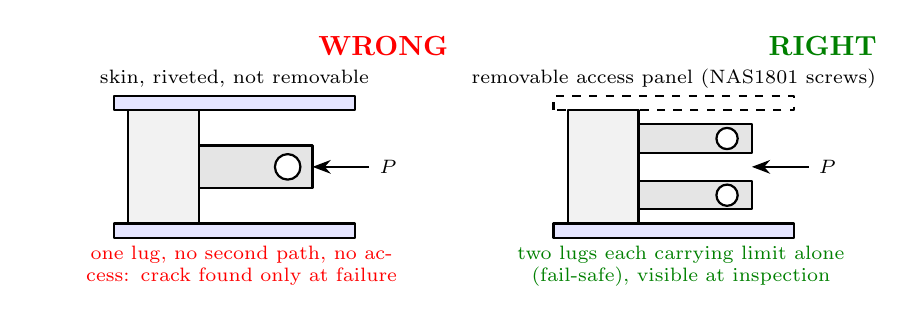
\begin{tikzpicture}[scale=0.9,>=Stealth,line join=round,font=\scriptsize]
% --- 10 wrong: single lug buried under skin
\begin{scope}
\draw[thick,fill=gray!10] (0,0) rectangle (1.0,1.6); % frame
\draw[thick,fill=gray!20] (1.0,0.5) -- (2.6,0.5) -- (2.6,1.1) -- (1.0,1.1) -- cycle; \draw[thick,fill=white] (2.25,0.8) circle (0.18);
\draw[thick,fill=blue!10] (-0.2,1.6) rectangle (3.2,1.8); \draw[thick,fill=blue!10] (-0.2,-0.2) rectangle (3.2,0);
\node at (1.5,2.05) {skin, riveted, not removable};
\draw[->,thick] (3.4,0.8) -- (2.6,0.8) node[pos=0,right] {$P$};
\node[red,capt] at (1.6,-0.6) {one lug, no second path, no access: crack found only at failure};
\node[red,font=\bfseries] at (3.6,2.5) {WRONG};
\end{scope}
\begin{scope}[xshift=6.2cm]
\draw[thick,fill=gray!10] (0,0) rectangle (1.0,1.6);
\draw[thick,fill=gray!20] (1.0,0.2) rectangle (2.6,0.6); \draw[thick,fill=white] (2.25,0.4) circle (0.15);
\draw[thick,fill=gray!20] (1.0,1.0) rectangle (2.6,1.4); \draw[thick,fill=white] (2.25,1.2) circle (0.15);
\draw[thick,fill=blue!10] (-0.2,-0.2) rectangle (3.2,0);
\draw[thick,dashed] (-0.2,1.6) rectangle (3.2,1.8); \node at (1.5,2.05) {removable access panel (NAS1801 screws)};
\draw[->,thick] (3.4,0.8) -- (2.6,0.8) node[pos=0,right] {$P$};
\node[green!50!black,capt] at (1.6,-0.6) {two lugs each carrying limit alone (fail-safe), visible at inspection};
\node[green!50!black,font=\bfseries] at (3.6,2.5) {RIGHT};
\end{scope}
\end{tikzpicture}
\end{frame}

\begin{frame}{Three accidents, three elements, three errors}
\begin{columns}[T]
\column{0.33\textwidth}
\textbf{de Havilland Comet, 1954}
\begin{itemize}
  \item Element: pressurised skin cut-out
  \item Error: square-cornered window, punched rivet holes
  \item Lesson: $K_t$ and pressurisation fatigue; full-scale fatigue test
\end{itemize}
\column{0.33\textwidth}
\textbf{Aloha Airlines 243, 1988}
\begin{itemize}
  \item Element: riveted lap joint with cold bond
  \item Error: bond failure shifted all load to rivets; multi-site cracking
  \item Lesson: multiple-site damage, inspection intervals
\end{itemize}
\column{0.33\textwidth}
\textbf{Alaska Airlines 261, 2000}
\begin{itemize}
  \item Element: stabiliser jackscrew and acme nut
  \item Error: wear without lubrication, no secondary load path
  \item Lesson: wear as a failure mode, maintenance in the design
\end{itemize}
\end{columns}
\vspace{6pt}
\begin{block}{}
None of these was a strength-margin error. All were element, detail, or maintenance errors --- the subject of this course.
\end{block}
\end{frame}

\section{Worked examples}

\begin{frame}{Example 1.1 -- Fuselage skin under cabin pressure}
$r=\SI{2.0}{m}$, $\Delta p=\SI{60}{kPa}$, 2024-T3 $t=\SI{1.6}{mm}$, $F_{tu}=434$, $F_{ty}=\SI{289}{MPa}$
\begin{align*}
\sigma_\theta &= \Delta p\,r/t = \SI{75}{MPa}\quad(\text{limit}), \qquad 1.5\sigma_\theta=\SI{112.5}{MPa}\\
\mathrm{MS}_{\text{ult}} &= 434/112.5-1 = 2.86, \qquad \mathrm{MS}_{\text{y}}=289/75-1=2.85
\end{align*}
\begin{alertblock}{Lesson}
Cabin skin is never sized by static strength. It is sized by crack growth from rivet holes over $\sim$60\,000 pressurisation cycles and by two-bay-crack residual strength. Static margins are necessary, rarely design-driving.
\end{alertblock}
\end{frame}

\begin{frame}{Example 1.2 -- Wing-attachment lug: fitting factor}
7075-T7351, $t=\SI{20}{mm}$, $d=\SI{25}{mm}$, $P_{\lim}=\SI{180}{kN}$; $F_{bru}=1055$, $F_{bry}=\SI{758}{MPa}$
\begin{align*}
P_u &= 1.5\times1.15\times180=\SI{310.5}{kN}\\
\sigma_{br} &= P_u/(dt)=\SI{621}{MPa},\qquad \mathrm{MS}_{\text{ult,br}}=1055/621-1=\mathbf{0.70}\\
\sigma_{br,\lim} &= 1.15\times180\,000/500=\SI{414}{MPa},\qquad \mathrm{MS}_{\text{y,br}}=758/414-1=\mathbf{0.83}
\end{align*}
\begin{itemize}
  \item Without the fitting factor: MS $=0.95$ --- on a fitting that is a certification finding
  \item Why does bearing \emph{yield} at limit matter for a pinned joint?
  \item Net section, shear-out and fatigue come later
\end{itemize}
\end{frame}

\begin{frame}{Example 1.3 -- Actuator rod end, combined loading}
$d=\SI{16}{mm}$, $P=\SI{25}{kN}$, $T=\SI{40}{N.m}$, 15-5PH $F_{ty}=\SI{1000}{MPa}$
\begin{align*}
\sigma_x &= 4P/\pi d^2=\SI{124.3}{MPa},\qquad \tau=16T/\pi d^3=\SI{49.7}{MPa}\\
\sigma' &= \sqrt{124.3^2+3(49.7)^2}=\SI{151.7}{MPa},\qquad \mathrm{MS}_{\text{y}}=1000/151.7-1=5.6
\end{align*}
Statically trivial. Sized later by fatigue at thread run-out ($K_t\approx3$--4) and by column buckling.
\end{frame}

\section{Next time}





\begin{frame}{For next time}
\begin{itemize}
  \item Read CS-25.301--25.307 (Subpart C, loads) and 25.601--25.625 (Subpart D, design and construction), each about one page, in the \href{https://www.easa.europa.eu/en/document-library/easy-access-rules/online-publications/easy-access-rules-large-aeroplanes-cs-25}{EASA Easy Access Rules for CS-25}; the American twin is \href{https://www.ecfr.gov/current/title-14/chapter-I/subchapter-C/part-25}{14 CFR Part 25 on the eCFR}
  \item Shigley Ch.\ 1, 3 (review), 5.1--5.5; Niu Ch.\ 1--3
  \item Self-study problems 1--5 in the notes
  \item Next: stress-life and strain-life fatigue --- the heart of the course
\end{itemize}
\end{frame}

\end{document}
